\documentclass[12pt,a4paper]{article}

% Biên dịch bằng pdfLaTeX: pdflatex ho-so-du-thi.tex
\usepackage[utf8]{inputenc}
\usepackage[T5]{fontenc}
\usepackage[vietnamese]{babel}
\usepackage[a4paper,left=30mm,right=25mm,top=25mm,bottom=25mm]{geometry}
\usepackage{lmodern}
\usepackage{graphicx}
\usepackage{booktabs}
\usepackage{longtable}
\usepackage{tabularx}
\usepackage{array}
\usepackage{multirow}
\usepackage{enumitem}
\usepackage{amsmath}
\usepackage{amssymb}
\usepackage[table]{xcolor}
\usepackage{float}
\usepackage{caption}
\usepackage{fancyhdr}
\usepackage{hyperref}
\usepackage{url}
\usepackage{microtype}

\definecolor{navy}{HTML}{17365D}
\definecolor{lightblue}{HTML}{EAF2F8}
\definecolor{lightgray}{HTML}{F3F4F6}
\definecolor{darkgray}{HTML}{3F4650}

\hypersetup{
  colorlinks=true,
  linkcolor=navy,
  urlcolor=navy,
  citecolor=navy,
  pdftitle={Hồ sơ dự án SafeViChi},
  pdfauthor={Đội phát triển SafeViChi}
}
\setlength{\parindent}{1.2em}
\setlength{\parskip}{0.35em}
\setlist{itemsep=0.25em,topsep=0.25em}
\captionsetup{font=small,labelfont=bf}
\newcolumntype{Y}{>{\raggedright\arraybackslash}X}
\newcommand{\projectname}{SafeViChi}
\newcommand{\missingcontent}{\textit{(Chưa bổ sung nội dung trong phiên bản hồ sơ này.)}}
\newcommand{\sourcepath}[1]{\texttt{\detokenize{#1}}}

\pagestyle{fancy}
\fancyhf{}
\fancyhead[L]{Hồ sơ dự án \projectname}
\fancyhead[R]{Sáng tạo trẻ quốc gia về trí tuệ nhân tạo}
\fancyfoot[C]{\thepage}
\setlength{\headheight}{15pt}

\begin{document}

\begin{titlepage}
  \centering
  \vspace*{10mm}
  {\Large\bfseries HỒ SƠ DỰ ÁN DỰ THI BẢNG C\par}
  \vspace{3mm}
  {\normalsize\itshape Cuộc thi Sáng tạo trẻ Quốc gia trong lĩnh vực Trí tuệ nhân tạo năm 2026\par}
  \vspace{6mm}
  {\large\bfseries Hệ thống phát hiện nội dung độc hại Tiếng Việt chống né lọc,\par
  xử lý cục bộ trên thiết bị\par}
  \vspace{7mm}
  \renewcommand{\arraystretch}{1.18}
  \small
  \begin{tabularx}{0.92\textwidth}{|p{0.42\textwidth}|X|}
    \hline
    \multicolumn{2}{|l|}{\textbf{Số lượng thí sinh trong đội thi:}\quad 1 người $\Box$\quad 2 người $\Box$\quad 3 người $\checkmark$}\\
    \hline
    \multicolumn{2}{|l|}{\cellcolor{lightblue}\textbf{Thí sinh thứ nhất (đội trưởng)}}\\
    \hline
    \textbf{Họ và tên:} & [Đã ẩn thông tin cá nhân]\\
    \hline
    \textbf{Ngày/tháng/năm sinh:} & [Đã ẩn]\\
    \hline
    \textbf{Lớp hành chính, ngành, khoa,\newline trường:} & K69A-AI2\\
    \hline
    \textbf{Xã/phường/đặc khu,\newline tỉnh/thành phố:} & [Đã ẩn]\\
    \hline
    \textbf{Điện thoại:} & [Đã ẩn]\\
    \hline
    \textbf{Email:} & [Đã ẩn]\\
    \hline
    \multicolumn{2}{|l|}{\cellcolor{lightblue}\textbf{Thí sinh thứ hai}}\\
    \hline
    \textbf{Họ và tên:} & [Đã ẩn thông tin cá nhân]\\
    \hline
    \textbf{Ngày/tháng/năm sinh:} & [Đã ẩn]\\
    \hline
    \textbf{Lớp hành chính, ngành, khoa,\newline trường:} & K69A-AI2\\
    \hline
    \textbf{Xã/phường/đặc khu,\newline tỉnh/thành phố:} & [Đã ẩn]\\
    \hline
    \textbf{Điện thoại:} & [Đã ẩn]\\
    \hline
    \textbf{Email:} & [Đã ẩn]\\
    \hline
    \multicolumn{2}{|l|}{\cellcolor{lightblue}\textbf{Thí sinh thứ ba}}\\
    \hline
    \textbf{Họ và tên:} & [Đã ẩn thông tin cá nhân]\\
    \hline
    \textbf{Ngày/tháng/năm sinh:} & [Đã ẩn]\\
    \hline
    \textbf{Lớp hành chính, ngành, khoa,\newline trường:} & K69A-AI4\\
    \hline
    \textbf{Xã/phường/đặc khu,\newline tỉnh/thành phố:} & [Đã ẩn]\\
    \hline
    \textbf{Điện thoại:} & [Đã ẩn]\\
    \hline
    \textbf{Email:} & [Đã ẩn]\\
    \hline
  \end{tabularx}
  \vfill
  {\normalsize Hà Nội, 2026}
\end{titlepage}

\pagenumbering{arabic}

\section{Bài toán hoặc vấn đề thực tiễn cần giải quyết}
Sự phát triển nhanh của mạng xã hội, diễn đàn và các nền tảng trao đổi trực tuyến làm tăng nhu cầu phát hiện sớm nội dung độc hại bằng tiếng Việt. Nội dung độc hại có thể gây tổn thương cho người bị hướng tới, tạo môi trường giao tiếp không an toàn và làm tăng khối lượng công việc kiểm duyệt. Trong nhóm người dùng trẻ, vấn đề càng đáng chú ý vì các em thường tiếp xúc với nội dung trực tuyến trước khi có đủ khả năng tự đánh giá rủi ro.

Một khó khăn kỹ thuật quan trọng là người viết có thể cố ý biến dạng câu chữ để né bộ lọc. Các hình thức thường gặp gồm bỏ dấu, dùng teencode, chèn khoảng trắng hoặc ký tự phân cách, kéo dài ký tự, thay ký tự bằng ký tự đồng dạng và kết hợp nhiều phép biến đổi trong cùng một câu. Những biến đổi này không nhất thiết làm thay đổi ý nghĩa đối với người đọc, nhưng làm thay đổi chuỗi đầu vào mà bộ phân loại nhận được. Mô hình chỉ được đánh giá trên câu viết chuẩn có thể vì vậy suy giảm mạnh khi đưa vào môi trường thực tế.

Một vấn đề thứ hai là yêu cầu bảo vệ nội dung riêng tư. Văn bản người dùng có thể chứa thông tin cá nhân, trao đổi gia đình hoặc nội dung nhạy cảm. Nếu phải gửi toàn bộ văn bản lên máy chủ bên ngoài để suy luận, hệ thống phát hiện có thể tạo thêm một rủi ro dữ liệu. SafeViChi giải quyết đồng thời hai yêu cầu: tăng độ bền trước biến dạng tiếng Việt và thực hiện suy luận cục bộ trên thiết bị.

Vấn đề thứ ba là khả năng kiểm tra lý do cảnh báo. Một nhãn HATE hoặc CLEAN đơn lẻ chưa cho biết phần nào trong câu đã làm mô hình đưa ra quyết định. Vì vậy, sản phẩm bổ sung module khoanh vùng bằng occlusion, nhằm chỉ ra các cụm từ có ảnh hưởng lớn đến điểm rủi ro. Kết quả này được dùng như thông tin hỗ trợ cho người giám sát, không thay thế quyết định của con người.

\section{Mục tiêu, phạm vi và đối tượng ứng dụng của sản phẩm}
\subsection{Mục tiêu}
Mục tiêu tổng quát của dự án là xây dựng một hệ thống phát hiện nội dung độc hại tiếng Việt có khả năng chống né lọc, trả về kết quả trên thiết bị và hỗ trợ giải thích. Mục tiêu được cụ thể hóa thành các yêu cầu sau:
\begin{enumerate}
  \item Tinh chỉnh ViHateT5 cho bài toán phân loại hai lớp CLEAN và HATE trên dữ liệu tiếng Việt có nhãn.
  \item Bổ sung lớp chuẩn hóa năm tầng để xử lý các biến dạng có thể mô tả bằng luật, gồm Unicode NFC, ký tự đồng dạng, ký tự phân cách, ký tự lặp và từ điển teencode.
  \item Sử dụng dữ liệu biến thể và huấn luyện đối kháng FGM để giảm suy giảm hiệu năng trên câu né lọc và câu điểm mù.
  \item Cung cấp điểm rủi ro, nhãn phân loại và vùng từ ngữ hỗ trợ giải thích bằng occlusion.
  \item Xuất mô hình sang ONNX và tích hợp với ONNX Runtime Web để minh họa khả năng xử lý cục bộ, không truyền văn bản người dùng lên máy chủ suy luận.
\end{enumerate}

\subsection{Phạm vi}
Phạm vi của phiên bản hiện tại là phát hiện nội dung thuộc hai lớp CLEAN và HATE trong văn bản tiếng Việt ngắn, đặc biệt là văn bản có các dạng biến đổi phi chuẩn thường gặp trên môi trường mạng. Hệ thống là một nguyên mẫu kỹ thuật có thể chạy trong trình duyệt; kết quả thực nghiệm dùng để chứng minh khả năng của phương pháp, chưa phải cam kết thay thế toàn bộ quy trình kiểm duyệt thương mại.

Hệ thống chưa thực hiện phân loại đầy đủ các nhóm độc hại khác nhau, chưa xác định danh tính người viết và không đưa ra quyết định xử phạt. Hệ thống cũng không tự động kết luận ý định của người dùng từ một câu đơn lẻ. Những giới hạn này được giữ rõ để tránh sử dụng điểm mô hình vượt quá phạm vi dữ liệu và mục tiêu đã đánh giá.

\subsection{Đối tượng ứng dụng}
\begin{itemize}
  \item \textbf{Phụ huynh và người giám hộ}: công cụ hỗ trợ xem xét nội dung có nguy cơ trong quá trình hướng dẫn trẻ, không phải công cụ đọc trộm hoặc giám sát tuyệt đối.
  \item \textbf{Trẻ em và thanh thiếu niên}: nhóm được bảo vệ, có thể được hưởng lợi từ cảnh báo sớm nhưng vẫn cần cơ chế giải thích và quyền được trao đổi với người lớn.
  \item \textbf{Nhà trường và tổ chức giáo dục}: nguyên mẫu phục vụ nghiên cứu an toàn số, kiểm thử chính sách và đào tạo nhận thức về nội dung độc hại.
  \item \textbf{Đơn vị xây dựng sản phẩm số}: mô hình kiến trúc có thể làm thành phần tiền xử lý và phát hiện cục bộ cho các ứng dụng cần giảm truyền dữ liệu văn bản.
\end{itemize}

\section{Dữ liệu sử dụng, nguồn dữ liệu và tính hợp lệ của dữ liệu}
\subsection{Các loại dữ liệu đã sử dụng}
Dự án sử dụng bốn nhóm dữ liệu chính:
\begin{enumerate}
  \item \textbf{Dữ liệu văn bản tiếng Việt có nhãn}: các mẫu CLEAN và HATE dùng để huấn luyện, validation và kiểm thử bộ phân loại.
  \item \textbf{Dữ liệu biến thể phi chuẩn}: các câu được tạo từ văn bản gốc bằng mười hai hiện tượng biến dạng có kiểm soát, bao gồm teencode, bỏ dấu, chèn ký tự phân tách, ký tự đồng dạng và lỗi gõ.
  \item \textbf{Dữ liệu điểm mù}: các biến thể được sinh với điều kiện sau chuẩn hóa, văn bản vẫn giữ nguyên hoặc gần như giữ nguyên. Nhóm này kiểm tra trường hợp lớp chuẩn hóa không đủ khả năng xử lý.
  \item \textbf{Dữ liệu giải thích}: tập ViHOS có nhãn vị trí từ ngữ độc hại do con người khoanh vùng, dùng để đánh giá module giải thích.
\end{enumerate}

\subsection{Nguồn dữ liệu và quy mô}
Các nguồn được ghi nhận trong mã nguồn và tệp dữ liệu gồm ViHSD, VOZ-HSD với nhãn yếu, và ViHOS từ kho \texttt{htdung167/ViHOS}. Dữ liệu sau khi dựng được lưu dưới dạng JSON Lines, kèm manifest mô tả nguồn, tỷ lệ trộn, seed và số lượng mẫu. Quy mô các tập chính được tổng hợp trong Bảng~\ref{tab:data-size}.

\begin{table}[H]
\centering
\caption{Quy mô dữ liệu sau khi tổ chức}
\label{tab:data-size}
\begin{tabularx}{\textwidth}{l r l X}
\toprule
\textbf{Tập} & \textbf{Số mẫu} & \textbf{Vai trò} & \textbf{Ghi chú}\\
\midrule
Huấn luyện & 116.943 & Tinh chỉnh mô hình & Trộn 60\% biến thể đã chuẩn hóa, 30\% câu gốc sạch, 10\% điểm mù.\\
Validation & 4.176 & Dò ngưỡng và dừng sớm & Tỷ lệ trộn tương ứng với tập huấn luyện; seed 42.\\
Test & 3.960 & Đánh giá cuối & Dùng sau khi ngưỡng đã được cố định.\\
ViHOS train & 8.844 & Phát triển module giải thích & Có nhãn câu và nhãn span.\\
ViHOS validation & 1.106 & Chọn ngưỡng giải thích & Có 537 câu HATE.\\
ViHOS test & 1.106 & Đánh giá khoanh vùng & Có 531 câu HATE.\\
\bottomrule
\end{tabularx}
\end{table}

\subsection{Hình thức thu thập và tổ chức}
Dữ liệu nguồn được tải từ các kho công khai đã được ghi trong cấu hình dựng dữ liệu. Dữ liệu biến thể không được thu thập trực tiếp từ người dùng; chúng được sinh tự động từ câu nguồn bằng trình sinh biến thể có kiểm soát trong \sourcepath{src/variant_generator/}. Dữ liệu được chia tách theo quy trình dựng tập, khử trùng lặp và lưu mã băm SHA-256 trong \sourcepath{data/CHECKSUMS.json}.

\subsection{Căn cứ về nguồn gốc, quyền sử dụng và quyền riêng tư}
Mỗi tập dữ liệu được lưu cùng thông tin nguồn trong manifest hoặc tài liệu kỹ thuật. Khi sử dụng dữ liệu nguồn, đội phát triển cần tuân thủ giấy phép và điều kiện truy cập của từng kho; hồ sơ nộp chính thức cần đính kèm bản sao hoặc đường dẫn giấy phép tương ứng. Dự án không đưa dữ liệu cá nhân mới vào hệ thống và không yêu cầu gửi văn bản người dùng lên máy chủ. Demo xử lý phía trình duyệt, do đó nội dung nhập được giữ trên thiết bị trong phạm vi phiên sử dụng. Các mẫu phát sinh chỉ dùng để huấn luyện và đánh giá, không dùng để suy ra danh tính cá nhân.

\subsection{Theo dõi nguồn gốc và kiểm soát tính hợp lệ}
Mỗi bản ghi trong pipeline được xem xét theo ba lớp thông tin. Lớp thứ nhất là thông tin nguồn, gồm tên bộ dữ liệu, phiên bản, split và nhãn ban đầu. Lớp thứ hai là thông tin biến đổi, gồm loại hiện tượng phi chuẩn, tham số sinh và văn bản trước và sau biến đổi. Lớp thứ ba là thông tin sử dụng, gồm tập train, validation hoặc test và bước xử lý đã áp dụng. Cách tổ chức này cho phép truy ngược một mẫu trong kết quả đánh giá về nguồn và phép biến đổi tương ứng.

Manifest của tập trộn ghi rõ tỷ lệ 60/30/10, seed 42, tổng số bản ghi và số trường hợp sinh điểm mù thất bại. Các số liệu này không chỉ phục vụ mô tả mà còn là điều kiện kiểm tra trước huấn luyện: nếu tổng số mẫu, tỷ lệ nguồn hoặc nhãn thay đổi ngoài dự kiến, lần chạy phải được xem là một phiên bản dữ liệu mới. Tệp mã băm SHA-256 được dùng để phát hiện việc sửa dữ liệu hoặc checkpoint sau khi đóng gói. Đây là cơ chế kiểm tra toàn vẹn, không thay thế cho việc kiểm tra giấy phép của dữ liệu nguồn.

\begin{table}[H]
\centering
\caption{Cơ cấu tập huấn luyện theo nguồn và nhãn}
\label{tab:train-composition}
\begin{tabular}{lrrr}
\toprule
\textbf{Nguồn} & \textbf{Tổng số} & \textbf{CLEAN} & \textbf{HATE}\\
\midrule
Biến thể đã chuẩn hóa & 70.166 & 35.869 & 34.297\\
Câu gốc sạch & 35.083 & 17.658 & 17.425\\
Điểm mù chưa chuẩn hóa & 11.694 & 5.886 & 5.808\\
\textbf{Tổng cộng} & \textbf{116.943} & \textbf{59.413} & \textbf{57.530}\\
\bottomrule
\end{tabular}
\end{table}

Tập huấn luyện có tỷ lệ hai nhãn gần cân bằng hơn so với validation và test, trong khi validation và test giữ phân bố tự nhiên của dữ liệu sau khi dựng. Điều này giúp quá trình học có đủ ví dụ HATE nhưng vẫn cho phép đánh giá ở một phân bố không được điều chỉnh thủ công. Riêng nhóm điểm mù có 4.476 trường hợp sinh thất bại ở tập huấn luyện; các trường hợp này không được coi là dữ liệu hợp lệ của nhóm điểm mù và được ghi lại để kiểm tra tỷ lệ thành công của bộ sinh.

\section{Quy trình tiền xử lý, làm sạch, chuẩn hóa hoặc tổ chức dữ liệu}
Quy trình tiền xử lý được tách thành các bước có thể tái lập:
\begin{enumerate}
  \item \textbf{Lựa chọn}: đọc dữ liệu theo schema thống nhất, giữ trường văn bản, nhãn, nguồn và thông tin biến thể cần cho kiểm tra.
  \item \textbf{Kiểm tra cấu trúc}: loại bản ghi thiếu văn bản hoặc nhãn, phát hiện span sai định dạng trong dữ liệu giải thích và ghi thống kê lỗi vào manifest.
  \item \textbf{Khử trùng lặp và chống rò rỉ}: so sánh các trường văn bản và tách dữ liệu theo quy trình cố định trước khi dựng benchmark.
  \item \textbf{Sinh biến thể}: áp dụng mười hai hiện tượng phi chuẩn theo seed đã ghi nhận. Mỗi biến thể được giữ thông tin truy nguyên về văn bản nguồn và phép biến đổi.
  \item \textbf{Chuẩn hóa}: áp dụng năm tầng gồm Unicode NFC, xử lý ký tự đồng dạng, xóa ký tự phân cách, gộp ký tự lặp và tra từ điển teencode.
  \item \textbf{Gán nhãn và trộn}: chuẩn hóa nhãn về hai lớp CLEAN và HATE; tập huấn luyện được trộn theo tỷ lệ 60/30/10 để mô hình đồng thời thấy biến thể có thể sửa, câu sạch và điểm mù.
  \item \textbf{Chuẩn bị đánh giá}: tạo ma trận C0, C1, C2 từ cùng nguồn câu để so sánh ghép cặp. Ngưỡng chỉ được dò trên validation và đóng băng trước khi chấm test.
\end{enumerate}

Bộ chuẩn hóa chỉ thay đổi bản sao đầu vào dùng cho mô hình. Văn bản hiển thị lại cho người dùng vẫn có thể giữ nguyên để phục vụ kiểm tra và giải thích. Các tệp trung gian, manifest và mã băm giúp kiểm tra lại đầu vào của từng lần chạy.

\subsection{Kiểm tra chất lượng trước khi đưa vào mô hình}
Trước khi tạo batch, mỗi bản ghi phải vượt qua các kiểm tra tối thiểu: trường văn bản không rỗng, nhãn thuộc tập giá trị cho phép, chuỗi có thể mã hóa bằng UTF-8 và không chứa dữ liệu cấu trúc bị hỏng. Với dữ liệu có span giải thích, chỉ số bắt đầu và kết thúc phải nằm trong phạm vi câu, không âm và không đảo ngược. Các bản ghi không hợp lệ được loại khỏi tập dùng cho mô hình nhưng số lượng và nguyên nhân bị loại vẫn được ghi trong manifest.

Một kiểm tra khác là đối chiếu văn bản sau chuẩn hóa với văn bản đầu vào. Nếu một luật làm thay đổi quá nhiều ký tự, mẫu được đưa vào nhóm cần xem xét vì có nguy cơ làm mất nghĩa. Các trường hợp chuẩn hóa không thay đổi văn bản được thống kê riêng; đây là nguồn đầu vào cho bộ sinh điểm mù và cũng là phép kiểm tra quan trọng về giới hạn của normalizer.

\subsection{Tách dữ liệu và chống rò rỉ}
Việc tách dữ liệu được thực hiện trước khi sinh các biến thể phụ thuộc vào câu nguồn, hoặc ít nhất phải bảo đảm các câu có cùng nguồn không xuất hiện ở cả train và test. Nếu một câu gốc nằm trong train nhưng biến thể của nó nằm trong test, mô hình có thể ghi nhớ nội dung thay vì học khả năng chống né lọc. Vì vậy, quy trình dựng dữ liệu giữ thông tin nguồn, thực hiện khử trùng lặp và kiểm tra giao giữa các split.

Tập validation được sử dụng để chọn ngưỡng và checkpoint; tập test chỉ được mở ở bước báo cáo cuối. Quy tắc này được áp dụng đồng nhất cho blacklist, mô hình gốc, mô hình có chuẩn hóa và mô hình tinh chỉnh đối kháng. Nhờ đó, so sánh giữa các hệ thống phản ánh khác biệt về phương pháp thay vì khác biệt về quyền truy cập vào test.

\subsection{Đầu ra của bước tiền xử lý}
Đầu ra gồm dữ liệu JSON Lines cho từng split, manifest tổng hợp, tệp đánh giá theo C0/C1/C2 và các mã băm. JSON Lines được chọn vì có thể đọc tuần tự, phù hợp với tập lớn và cho phép kiểm tra từng bản ghi. Manifest được lưu ở dạng JSON để các script đánh giá có thể đọc trực tiếp số lượng, tỷ lệ nguồn, seed và tình trạng sinh dữ liệu. Cấu trúc này giúp tách dữ liệu khỏi mã huấn luyện, nhờ đó có thể tái lập thí nghiệm mà không cần chạy lại toàn bộ bước sinh biến thể.

\subsection{Chi tiết năm tầng chuẩn hóa}
Năm tầng được sắp xếp theo mức độ tổng quát tăng dần. Unicode NFC xử lý các cách biểu diễn tương đương về mặt mã hóa. Tầng ký tự đồng dạng đưa một số ký tự có hình thức gần nhau về dạng được mô hình biết. Tầng xóa phân cách xử lý các dấu chấm, khoảng trắng hoặc ký hiệu được chèn giữa các ký tự. Tầng gộp ký tự lặp giảm tác động của việc kéo dài một ký tự nhiều lần. Cuối cùng, từ điển teencode thay thế các dạng viết tắt đã được xác định bằng quy tắc.

Mỗi tầng phải có kiểm thử độc lập và kiểm thử kết hợp. Việc tách tầng giúp xác định trường hợp một phép biến đổi làm thay đổi nhãn, đồng thời tránh việc một luật quá rộng xóa mất thông tin ngữ nghĩa. Các luật không được coi là bộ lọc độc lập; chúng chỉ tạo đầu vào nhất quán hơn cho mô hình học sâu. Những mẫu không được sửa hoặc cố tình giữ nguyên sau chuẩn hóa được chuyển sang nhóm điểm mù để đánh giá riêng.

\begin{table}[H]
\centering
\caption{Nhóm hiện tượng phi chuẩn được mô phỏng}
\label{tab:perturbations}
\begin{tabularx}{\textwidth}{p{0.28\textwidth}p{0.47\textwidth}p{0.17\textwidth}}
\toprule
\textbf{Nhóm biến đổi} & \textbf{Mục đích kiểm tra} & \textbf{Khả năng xử lý chính}\\
\midrule
Teencode và viết tắt & Mô phỏng cách viết nhanh, thay chữ hoặc thay âm trong hội thoại trực tuyến. & Từ điển và mô hình\\
Bỏ dấu hoặc thay dấu & Kiểm tra độ phụ thuộc của mô hình vào dấu tiếng Việt. & Chuẩn hóa và mô hình\\
Chèn phân cách & Chia nhỏ từ hoặc cụm từ bằng khoảng trắng, dấu câu hoặc ký hiệu. & Xóa phân cách\\
Ký tự đồng dạng & Thay ký tự bằng hình thức tương tự trong bảng mã khác. & Unicode và mô hình\\
Lặp ký tự, lỗi gõ & Kéo dài ký tự hoặc tạo sai lệch giống lỗi nhập liệu. & Gộp lặp và mô hình\\
Biến thể hỗn hợp & Kết hợp nhiều hiện tượng trong cùng một câu. & Đối kháng\\
\bottomrule
\end{tabularx}
\end{table}

Các nhóm trên được dùng để kiểm tra cả hai khả năng: hệ thống sửa được biến thể đã biết và hệ thống vẫn nhận diện được biến thể chưa được mô tả đầy đủ bằng luật. Trong quá trình dựng dữ liệu, nhãn ngữ nghĩa của câu nguồn được giữ lại cho câu biến thể, nhưng văn bản biến thể và lịch sử phép biến đổi được lưu riêng để không làm mất khả năng phân tích lỗi.

\section{Thuật toán, mô hình, phương pháp hoặc công cụ trí tuệ nhân tạo được sử dụng}
\begin{table}[H]
\centering
\caption{Các thành phần trí tuệ nhân tạo và vai trò}
\label{tab:components}
\begin{tabularx}{\textwidth}{p{0.27\textwidth}p{0.65\textwidth}}
\toprule
\textbf{Thành phần} & \textbf{Vai trò trong hệ thống}\\
\midrule
Bộ chuẩn hóa theo luật & Giảm các biến dạng có quy tắc trước khi phân loại; hoạt động nhanh và có thể kiểm tra từng tầng.\\
ViHateT5 & Mô hình ngôn ngữ nền cho phân loại hai lớp CLEAN/HATE trong tiếng Việt.\\
Fine-tune & Điều chỉnh ViHateT5 trên dữ liệu của dự án để học nhãn và phân bố biến thể mục tiêu.\\
FGM & Tạo nhiễu đối kháng trên embedding trong huấn luyện, tăng khả năng chịu các biến dạng chưa được chuẩn hóa hết.\\
Occlusion với cửa sổ 2 từ & Che lần lượt từng cụm hai từ, tính mức giảm logit margin và trả về các vị trí gây ảnh hưởng lớn.\\
ONNX Runtime Web & Chạy mô hình đã xuất ONNX trực tiếp trong trình duyệt, không cần dịch vụ suy luận phía máy chủ.\\
Blacklist từ khóa & Mô hình cơ sở để đánh giá mức cải thiện của hệ thống học sâu và lớp chuẩn hóa.\\
\bottomrule
\end{tabularx}
\end{table}

Luồng tính điểm phân loại dùng nhãn do mô hình sinh ra và ngưỡng được chọn trên validation. Với module giải thích, điểm của một cửa sổ được xác định dựa trên thay đổi của logit margin thay vì thay đổi xác suất, vì xác suất có thể bão hòa về 1 trong các câu độc hại rõ ràng.

\subsection{Quan hệ giữa các thành phần}
Bộ chuẩn hóa là thành phần xác định, có thể kiểm tra bằng các ca kiểm thử đầu vào--đầu ra. ViHateT5 đảm nhiệm phần suy luận theo ngữ cảnh, trong đó cùng một từ có thể mang mức rủi ro khác nhau tùy câu. FGM bổ sung nhiễu trong giai đoạn huấn luyện chứ không được gọi như một bước xử lý khi người dùng nhập câu. Occlusion được chạy sau phân loại và chỉ dùng để giải thích, vì vậy kết quả khoanh vùng không được hiểu là một nhãn mới.

Thiết kế này tạo ra ranh giới rõ giữa tiền xử lý, suy luận và giải thích. Khi thay đổi từ điển hoặc luật chuẩn hóa, có thể đánh giá lại tầng tiền xử lý mà không cần thay đổi checkpoint. Khi thay đổi mô hình, giao diện vẫn giữ hợp đồng đầu ra gồm nhãn, điểm rủi ro và vùng cảnh báo. Khi module giải thích không đủ tin cậy, nhãn phân loại vẫn có thể được sử dụng độc lập nhưng giao diện cần thông báo rõ rằng vùng tô sáng là kết quả hỗ trợ kiểm tra.

\subsection{Cơ sở lựa chọn mô hình nền}
ViHateT5 được chọn vì đã có năng lực xử lý tiếng Việt và có thể được tinh chỉnh theo định dạng nhãn của dự án. Sử dụng mô hình nền giúp giảm chi phí học từ đầu và tập trung nguồn lực vào vấn đề chính là biến dạng văn bản. Tuy nhiên, mô hình nền không được coi là đã chống né lọc; kết quả C1 của mô hình gốc cho thấy khả năng ngôn ngữ chung không đủ để xử lý mọi thay đổi hình thức.

\subsection{Bộ cơ sở và các cấu hình đối chứng}
Blacklist từ khóa được dùng làm mốc chi phí thấp. ViHateT5 gốc cho biết mức hiệu năng khi chỉ dùng mô hình nền. ViHateT5 gốc cộng chuẩn hóa đo đóng góp của luật tiền xử lý. ViHateT5 tinh chỉnh đối kháng nhưng không chuẩn hóa đo đóng góp riêng của dữ liệu và FGM. Cấu hình đầy đủ kết hợp tất cả thành phần. Các cấu hình này tạo thành phép thử loại bỏ thành phần, hỗ trợ kết luận về nguyên nhân của mức cải thiện.

Một thành phần được xem là có đóng góp khi việc thêm thành phần tạo ra thay đổi ổn định trên cùng ma trận dữ liệu và không làm suy giảm không thể chấp nhận ở C0. Cách đánh giá này tránh việc chỉ chọn thành phần vì một điểm số tốt nhất trên một điều kiện. Nó cũng cho phép xác định giới hạn: normalizer có thể xử lý biến thể theo luật, nhưng không đảm bảo xử lý được điểm mù; mô hình đối kháng có thể cải thiện C2, nhưng vẫn cần lớp chuẩn hóa để đạt kết quả cao nhất trên C1.

\section{Quy trình huấn luyện, tinh chỉnh, tích hợp hoặc khai thác mô hình}
\subsection{Đầu vào và thiết lập huấn luyện}
Mô hình nhận văn bản đã được hạ chữ thường trước khi đưa vào tokenizer. Tập huấn luyện gồm 116.943 mẫu theo tỷ lệ 60/30/10. ViHateT5 được tinh chỉnh với learning rate $10^{-5}$, tám epoch tối đa, FGM với $\epsilon=0.3$, batch 16 trên mỗi thiết bị, bật FP16 khi phần cứng hỗ trợ. Huấn luyện dùng seed 42 và early stopping với patience bằng 2 epoch.

Việc hạ chữ thường là cần thiết vì tokenizer của mô hình nền có giới hạn với ký tự hoa. Nội dung nguyên bản vẫn được lưu cho giao diện và đối chiếu; chỉ chuỗi đưa vào tokenizer được xử lý.

Quy trình huấn luyện bắt đầu bằng việc đọc manifest và kiểm tra kích thước tập. Sau đó dữ liệu được mã hóa bằng tokenizer, tạo batch và đưa qua mô hình nền. Ở mỗi bước huấn luyện thông thường, loss được tính từ nhãn CLEAN/HATE. Với bước đối kháng, gradient của batch được dùng để tạo nhiễu nhỏ trên embedding, mô hình được chạy lại trên biểu diễn nhiễu và loss được cộng vào quá trình cập nhật. Nhiễu được khôi phục sau mỗi bước để không làm thay đổi trọng số theo cách ngoài thiết kế.

Việc chọn checkpoint không dựa trên một nhóm biến thể riêng. Validation được trộn tương ứng với dữ liệu huấn luyện, nhờ đó checkpoint được chọn trên phân bố gần với tình huống triển khai. Đây là điểm quan trọng vì trong thực tế hệ thống không biết trước một câu đến là C0, C1 hay C2. Dùng validation riêng cho từng điều kiện có thể tạo ra ngưỡng tối ưu giả tạo và không phản ánh cách vận hành chung.

\subsection{Kiểm tra và điều chỉnh}
Validation được dùng cho hai mục đích: theo dõi F1 để chọn checkpoint tốt nhất và dò ngưỡng phân loại. Sau khi chọn ngưỡng, ngưỡng này được giữ cố định cho cả C0, C1 và C2 trên test. Không dùng kết quả test để điều chỉnh lại mô hình hoặc ngưỡng.

Trong mỗi lần chạy, cần lưu learning rate, epsilon đối kháng, kích thước batch, số epoch, patience, seed, tên checkpoint nền và đường dẫn dữ liệu. Đây là các tham số có thể làm thay đổi kết quả dù mã nguồn không đổi. Khi F1 validation không cải thiện trong số epoch quy định, early stopping dừng huấn luyện và giữ checkpoint tốt nhất thay vì checkpoint cuối cùng. Cách này làm giảm nguy cơ chọn một trạng thái đã bắt đầu quá khớp với validation.

\subsection{Kiểm tra sau huấn luyện}
Sau khi chọn checkpoint, mô hình được kiểm tra trên một tập nhỏ trước khi chạy toàn bộ benchmark. Smoke test xác nhận tokenizer, kích thước đầu vào, nhãn đầu ra, thiết bị tính toán và đường dẫn checkpoint. Tiếp theo, đánh giá đầy đủ tạo scores cho từng điều kiện và ghi thời gian suy luận. Nếu checkpoint thiếu tệp tokenizer hoặc cấu hình, quy trình phải dừng thay vì tự tải một tệp khác không được ghi nhận.

Khi xuất ONNX, kết quả của một số câu đại diện được so sánh với mô hình gốc. Các câu đại diện cần bao phủ cả trường hợp mô hình dự đoán CLEAN, HATE, câu né lọc và câu có giải thích. Sai khác nhỏ do kiểu số có thể chấp nhận trong ngưỡng đã quy định, nhưng thay đổi nhãn hoặc vùng cảnh báo phải được xem xét trước khi phát hành.

\subsection{Tích hợp sản phẩm}
Checkpoint tốt nhất được xuất sang ONNX để chạy trong trình duyệt. Phía trình duyệt thực hiện chuẩn hóa, tokenization và suy luận bằng ONNX Runtime Web. Module giải thích chạy sau khi có kết quả HATE, sử dụng occlusion để khoanh vùng từ ngữ. Toàn bộ pipeline đầu-cuối được đóng gói trong \sourcepath{src/pipeline.py}; ứng dụng demo nằm trong thư mục \sourcepath{demo/}.

Trước khi xuất mô hình, cần kiểm tra sự tương đương giữa đầu ra PyTorch và đầu ra ONNX trên một tập câu cố định. Tập kiểm tra này nên bao gồm câu sạch, câu có dấu, câu không dấu, teencode, ký tự đồng dạng và câu có ký tự lặp. Sai khác nhỏ do kiểu số có thể chấp nhận trong ngưỡng đã quy định, nhưng thay đổi nhãn hoặc vùng cảnh báo phải được xem xét trước khi phát hành. Bản demo cũng cần kiểm tra trường hợp mô hình chưa tải xong, văn bản rỗng, văn bản quá dài và lỗi tải tài nguyên.

\section{Chỉ số, phương pháp hoặc tiêu chí đánh giá kết quả}
Chỉ số chính của bộ phân loại là F1 của lớp HATE, vì bài toán cần cân bằng giữa phát hiện đúng nội dung độc hại và hạn chế bỏ sót. Báo cáo bổ sung Precision, Recall, accuracy, macro F1 và khoảng tin cậy của F1. Module giải thích được đánh giá bằng micro F1 theo từ, macro F1 theo câu, Precision, Recall, tỷ lệ câu không khoanh trúng từ nào và tỷ lệ câu có F1 từ 0,5 trở lên.

Đánh giá được thực hiện trên ma trận ba điều kiện:
\begin{itemize}
  \item C0: câu sạch, chưa biến dạng;
  \item C1: câu đã qua biến dạng né lọc;
  \item C2: câu điểm mù, được tạo để lớp chuẩn hóa không thể sửa trực tiếp.
\end{itemize}

Ngoài so sánh số học, dự án dùng kiểm định McNemar ghép cặp để kiểm tra sự khác biệt giữa các hệ thống trên cùng mẫu. Ngưỡng thống kê được báo cáo trong tài liệu thực nghiệm là $p<10^{-6}$ đối với các kết luận chính.

Với một lớp nhị phân, Precision được tính bằng $TP/(TP+FP)$ và Recall bằng $TP/(TP+FN)$. F1 được ưu tiên vì chỉ số này giảm khi một hệ thống chỉ tối ưu một phía: chỉ tăng Recall nhưng tạo quá nhiều cảnh báo giả hoặc chỉ tăng Precision nhưng bỏ sót nhiều nội dung độc hại. Macro F1 được tính bằng cách lấy trung bình giữa các lớp hoặc giữa các câu theo thiết lập tương ứng; nó giúp tránh việc kết quả bị chi phối hoàn toàn bởi lớp CLEAN có số lượng lớn hơn.

Giao thức đánh giá gồm bốn bước. Thứ nhất, dựng cùng một ma trận dữ liệu cho mọi hệ thống cơ sở. Thứ hai, chạy validation để dò ngưỡng. Thứ ba, cố định ngưỡng và chạy test một lần cho từng hệ thống. Thứ tư, lưu số liệu, cấu hình, seed và biểu đồ. Khoảng tin cậy của F1 giúp thể hiện độ bất định do kích thước mẫu; kiểm định ghép cặp giúp trả lời liệu chênh lệch quan sát được có vượt quá dao động ngẫu nhiên trên cùng dữ liệu hay không.

\begin{table}[H]
\centering
\caption{Các tiêu chí đánh giá theo mục tiêu sử dụng}
\label{tab:evaluation-criteria}
\begin{tabularx}{\textwidth}{p{0.25\textwidth}p{0.28\textwidth}p{0.37\textwidth}}
\toprule
\textbf{Mục tiêu} & \textbf{Chỉ số chính} & \textbf{Cách diễn giải}\\
\midrule
Phát hiện HATE & F1 lớp HATE & Cân bằng giữa bỏ sót nội dung độc hại và cảnh báo nhầm.\\
Không bỏ sót & Recall lớp HATE & Cho biết tỷ lệ nội dung HATE được phát hiện.\\
Giảm cảnh báo nhầm & Precision lớp HATE & Cho biết tỷ lệ cảnh báo thực sự thuộc lớp HATE.\\
Độ ổn định theo lớp & Macro F1, accuracy & Kiểm tra ảnh hưởng của mất cân bằng nhãn.\\
Chống né lọc & F1 theo C0/C1/C2 & Đo riêng khả năng chịu biến dạng và điểm mù.\\
Giải thích & Micro F1, Macro F1, tỷ lệ trượt & Đo khả năng khoanh đúng vùng từ ngữ được gán nhãn.\\
\bottomrule
\end{tabularx}
\end{table}

Kết quả định lượng cần được đọc cùng điều kiện tạo ra nó. F1 C1 chỉ có ý nghĩa khi số lượng mẫu, kiểu biến dạng, ngưỡng và cách chia dữ liệu được công bố. Tương tự, điểm giải thích trên ViHOS chỉ phản ánh nhiệm vụ khoanh vùng theo nhãn span của tập đó, không thể diễn giải thành khả năng giải thích cho mọi loại nội dung độc hại. Hồ sơ vì vậy tách rõ kết quả phân loại và kết quả giải thích.

\section{Kết quả thử nghiệm, phân tích ưu điểm, hạn chế và khả năng mở rộng}
\subsection{Kết quả phân loại}
Bảng~\ref{tab:f1-results} trình bày F1 của lớp HATE trên tập test. Các hệ thống được đánh giá trên cùng điều kiện và dùng ngưỡng đã dò từ validation.

\begin{table}[H]
\centering
\caption{F1 lớp HATE trên ba điều kiện test}
\label{tab:f1-results}
\begin{tabular}{lccc}
\toprule
\textbf{Hệ thống} & \textbf{C0} & \textbf{C1} & \textbf{C2}\\
\midrule
Blacklist từ khóa & 0,6551 & 0,5982 & 0,4564\\
ViHateT5 gốc & 0,7683 & 0,6046 & 0,4627\\
ViHateT5 gốc + chuẩn hóa & 0,7497 & 0,7218 & 0,4720\\
ViHateT5 tinh chỉnh đối kháng & 0,8523 & 0,7441 & 0,6657\\
\textbf{SafeViChi đầy đủ} & \textbf{0,8552} & \textbf{0,8266} & \textbf{0,6657}\\
\bottomrule
\end{tabular}
\end{table}

\begin{figure}[H]
\centering
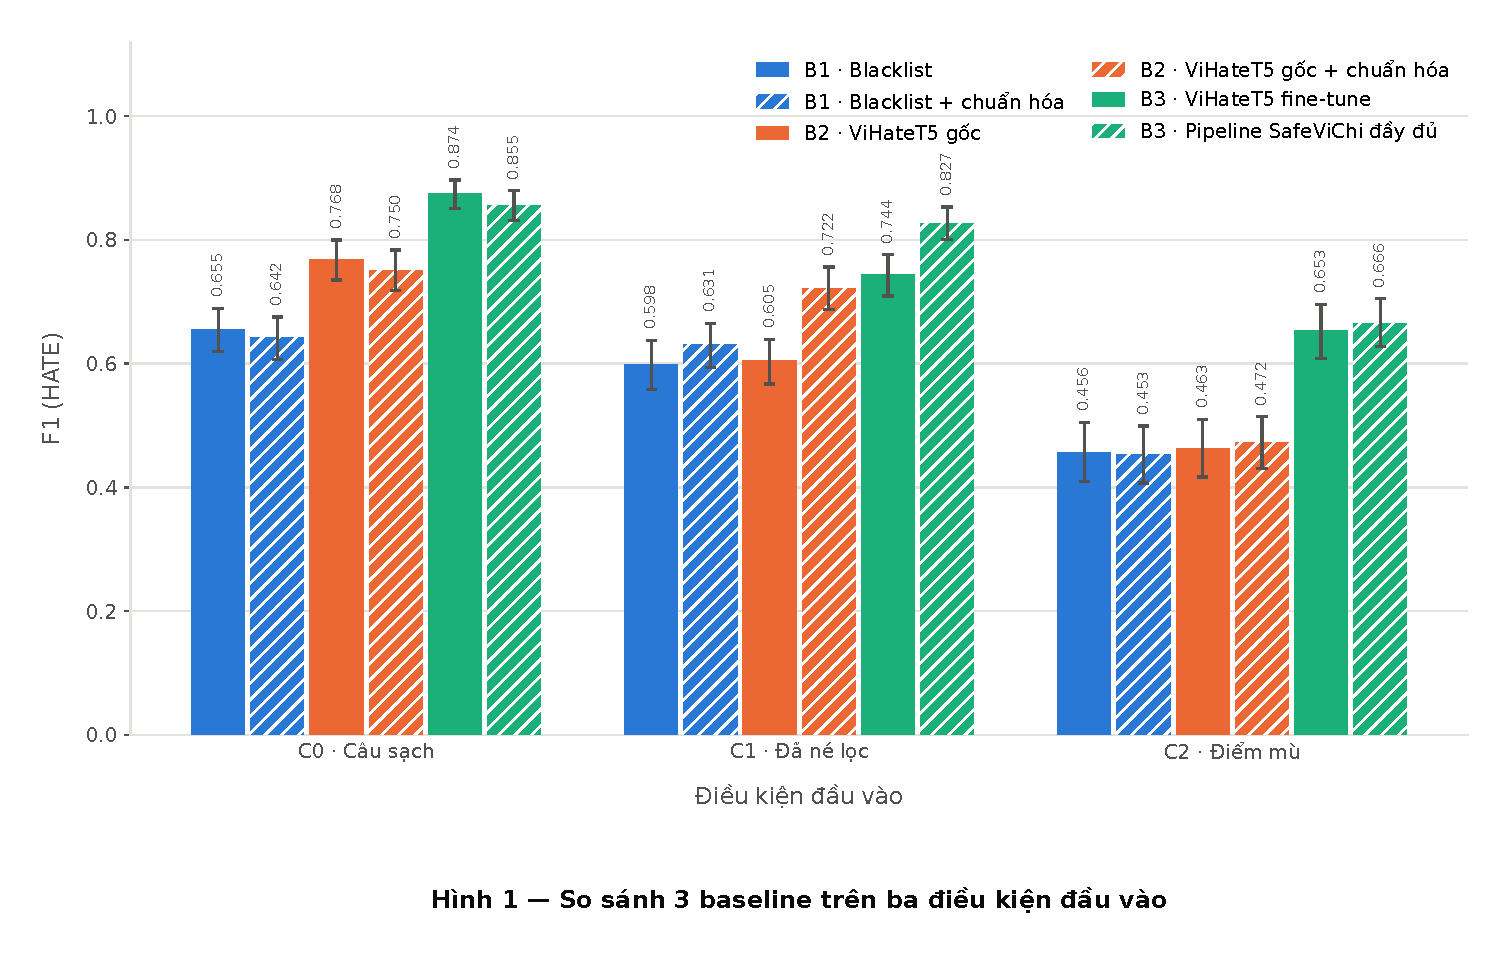
\includegraphics[width=0.88\textwidth]{../results/step3/figures/hinh1_ma_tran_f1.pdf}
\caption{Ma trận F1 theo hệ thống và điều kiện đánh giá}
\label{fig:f1-matrix}
\end{figure}

So với ViHateT5 gốc, SafeViChi đầy đủ tăng F1 trên C1 từ 0,6046 lên 0,8266, tương đương tăng 0,2220 điểm tuyệt đối. Trên C2, F1 tăng từ 0,4627 lên 0,6657, cho thấy huấn luyện đối kháng xử lý được một phần biến dạng mà bộ chuẩn hóa không nhận diện. Trên C0, F1 đạt 0,8552, nên việc bổ sung khả năng chống né lọc không chỉ giới hạn ở dữ liệu biến dạng.

Hình~\ref{fig:f1-matrix} cho thấy sự khác biệt giữa các hệ thống không chỉ xuất hiện trên một điều kiện. Blacklist có hiệu năng thấp nhất ở C2 vì phụ thuộc vào sự xuất hiện nguyên dạng của từ khóa. ViHateT5 gốc có lợi thế trên câu sạch nhưng suy giảm mạnh khi hình thức câu thay đổi. SafeViChi giữ được mức F1 cao hơn trên cả ba cột, trong đó khoảng cách với mô hình gốc lớn nhất ở C1 và C2.

\begin{figure}[H]
\centering
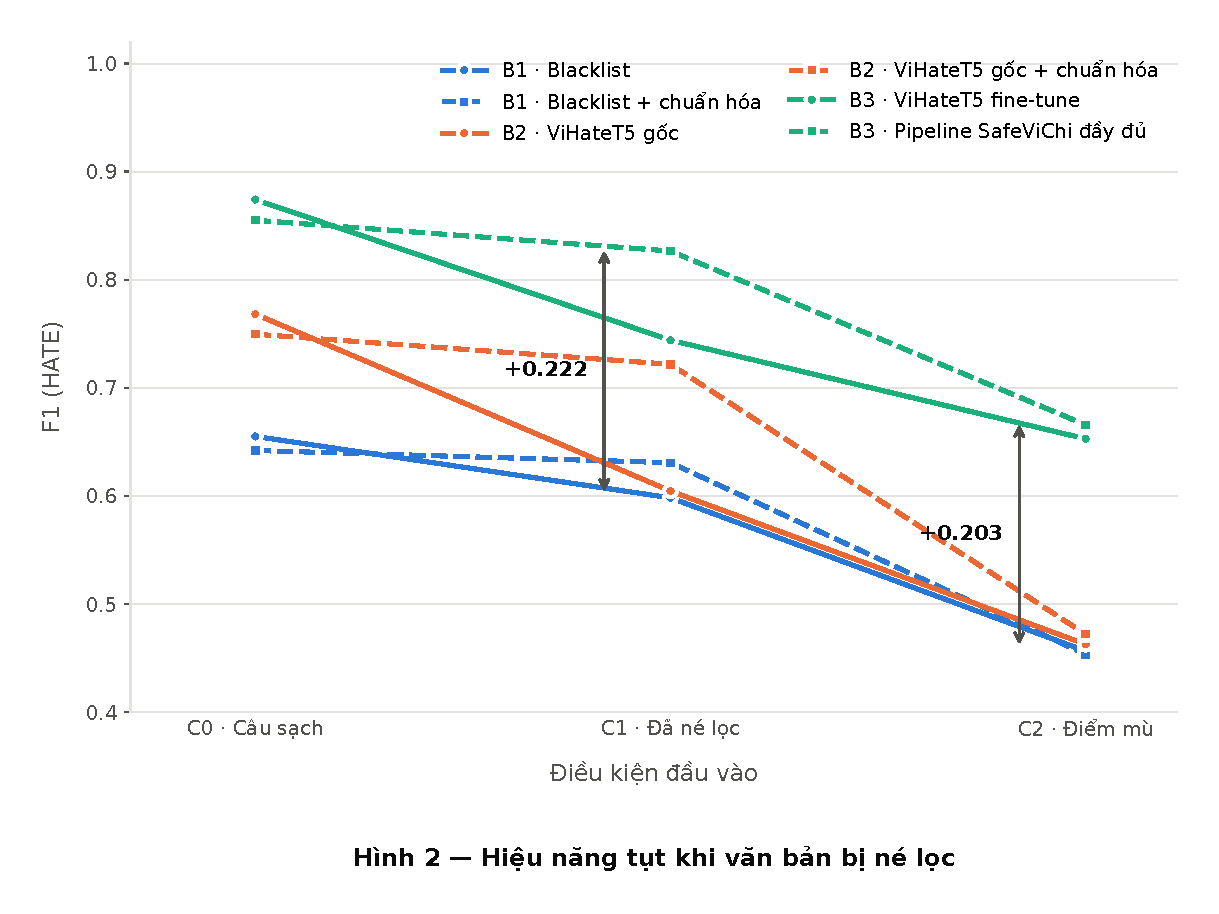
\includegraphics[width=0.88\textwidth]{../results/step3/figures/hinh2_do_tut_hieu_nang.pdf}
\caption{Mức sụt giảm hiệu năng khi chuyển từ câu sạch sang câu né lọc}
\label{fig:performance-drop}
\end{figure}

Hình~\ref{fig:performance-drop} bổ sung góc nhìn theo mức suy giảm thay vì chỉ nhìn điểm F1 tuyệt đối. ViHateT5 gốc chịu ảnh hưởng lớn khi chuyển từ C0 sang C1. Lớp chuẩn hóa làm giảm phần suy giảm do các biến dạng đã biết; huấn luyện đối kháng tiếp tục giảm phụ thuộc vào hình thức bề mặt. Trên C2, kết quả vẫn thấp hơn C0 vì đây là nhóm được thiết kế để vượt qua lớp luật, nhưng mô hình đối kháng phục hồi đáng kể so với mô hình gốc.

\begin{figure}[H]
\centering
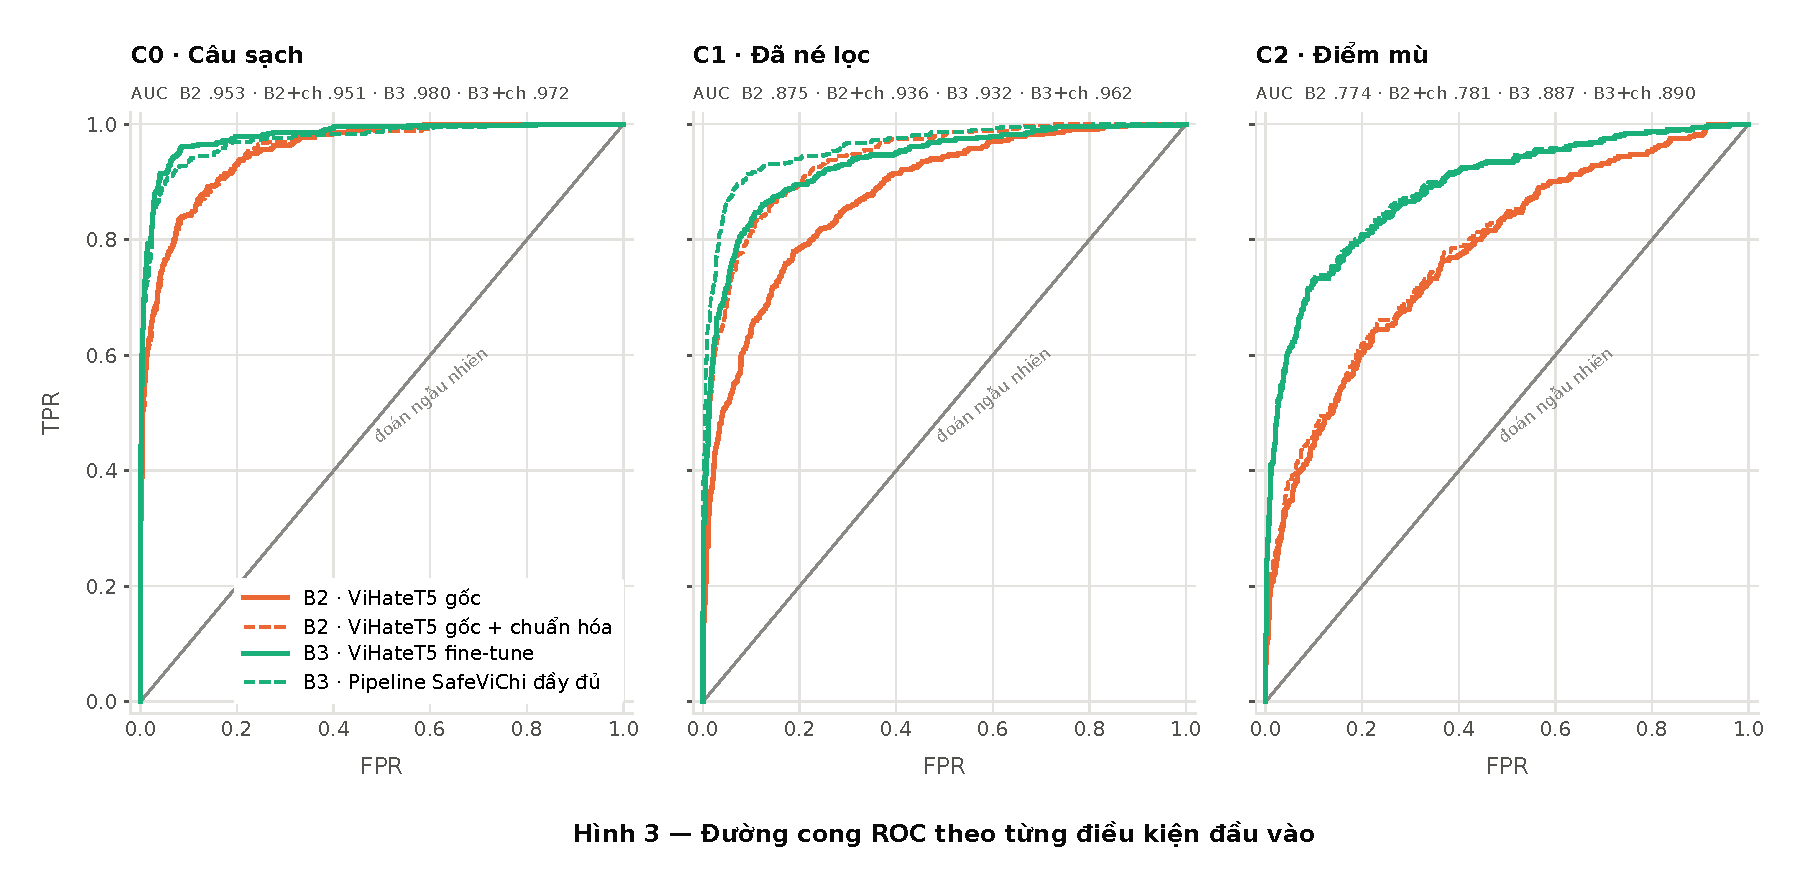
\includegraphics[width=0.88\textwidth]{../results/step3/figures/hinh3_duong_cong_roc.pdf}
\caption{Đường cong ROC của các hệ thống trên ma trận đánh giá}
\label{fig:roc}
\end{figure}

Đường cong ROC trong Hình~\ref{fig:roc} cho biết hành vi của hệ thống khi thay đổi ngưỡng, không chỉ tại ngưỡng cuối cùng được chọn. Đây là kiểm tra bổ sung cho F1: một mô hình có đường cong tốt hơn thường có nhiều vùng lựa chọn cân bằng giữa tỷ lệ phát hiện đúng và tỷ lệ cảnh báo nhầm. Tuy nhiên, khi triển khai, hệ thống vẫn phải dùng một ngưỡng đã chọn từ validation thay vì chọn lại theo loại câu quan sát được.

\begin{figure}[H]
\centering
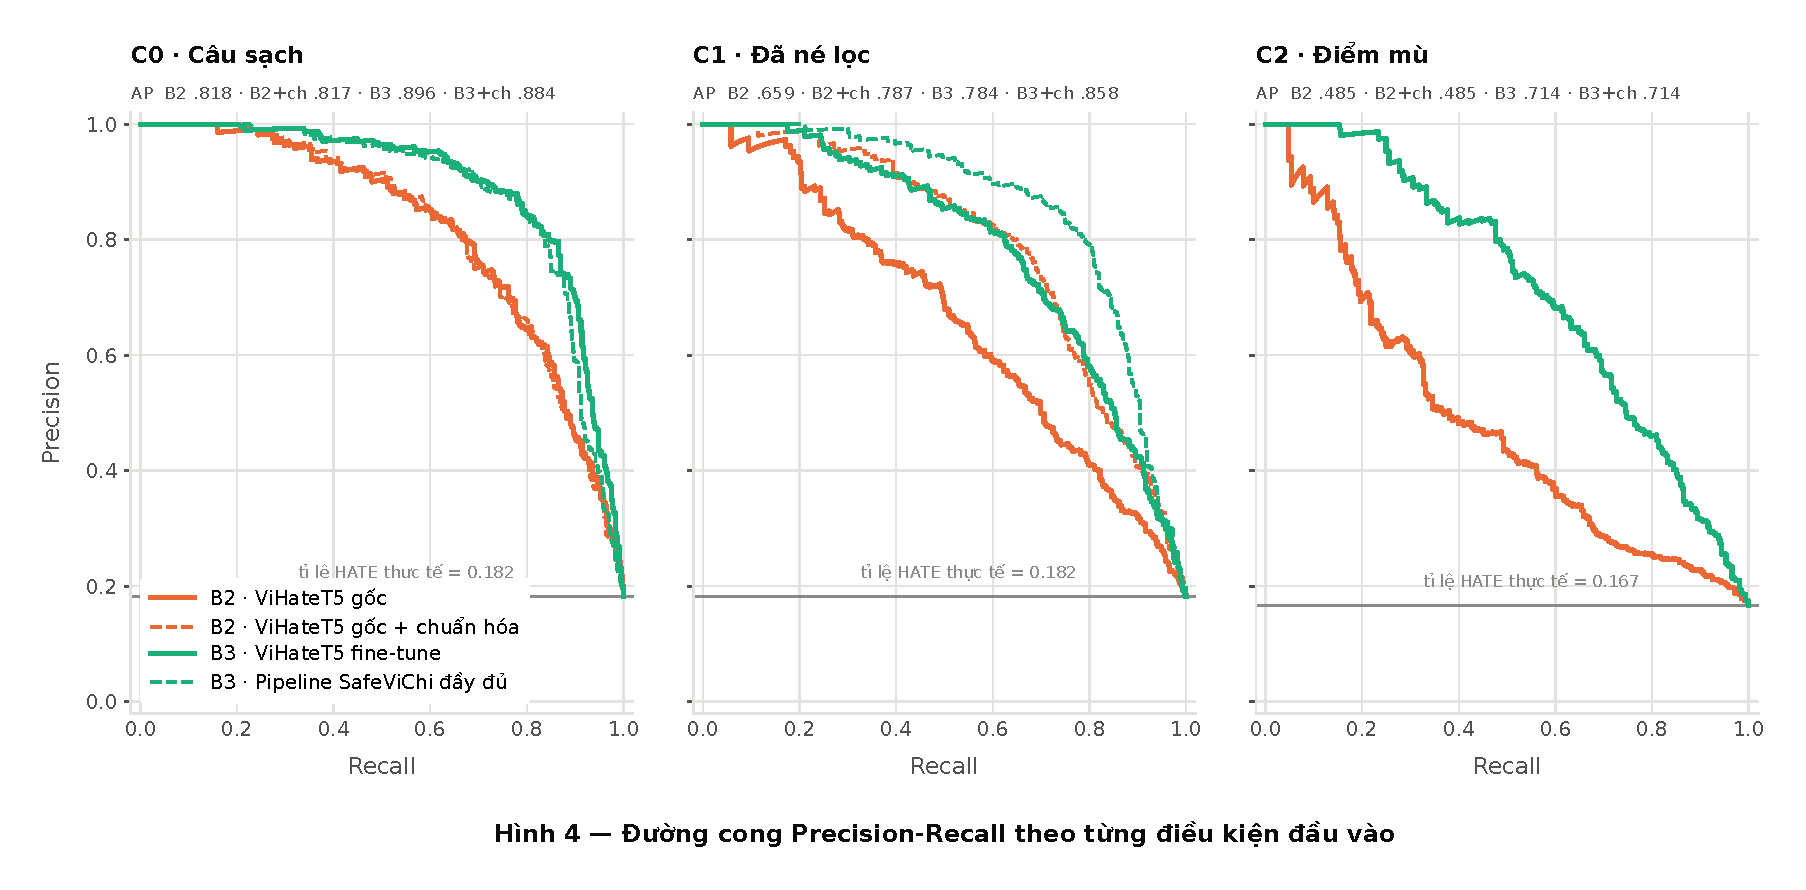
\includegraphics[width=0.88\textwidth]{../results/step3/figures/hinh4_duong_cong_pr.pdf}
\caption{Đường cong Precision--Recall của các hệ thống}
\label{fig:pr}
\end{figure}

Hình~\ref{fig:pr} phù hợp hơn ROC khi quan tâm trực tiếp đến lớp HATE có tỷ lệ nhỏ hơn lớp CLEAN. Đường cong thể hiện chi phí của việc tăng Recall: hệ thống có thể phát hiện thêm nội dung độc hại nhưng đồng thời tạo thêm cảnh báo giả. Vì vậy, F1 và điểm vận hành cụ thể cần được báo cáo cùng nhau, thay vì chỉ chọn mô hình dựa trên một điểm của đường cong.

\subsection{Kết quả giải thích}
Trên 531 câu HATE của ViHOS test, module occlusion đạt micro F1 0,5455, Precision 0,4478, Recall 0,6977 và macro F1 0,5766 theo báo cáo thực nghiệm. Tỷ lệ trượt hoàn toàn được ghi nhận là 1,9\%; 67,2\% câu đạt F1 từ 0,5 trở lên. Recall cao hơn Precision, phù hợp với việc cửa sổ hai từ có thể mở rộng vùng dự đoán sang các từ lân cận.

\begin{figure}[H]
\centering
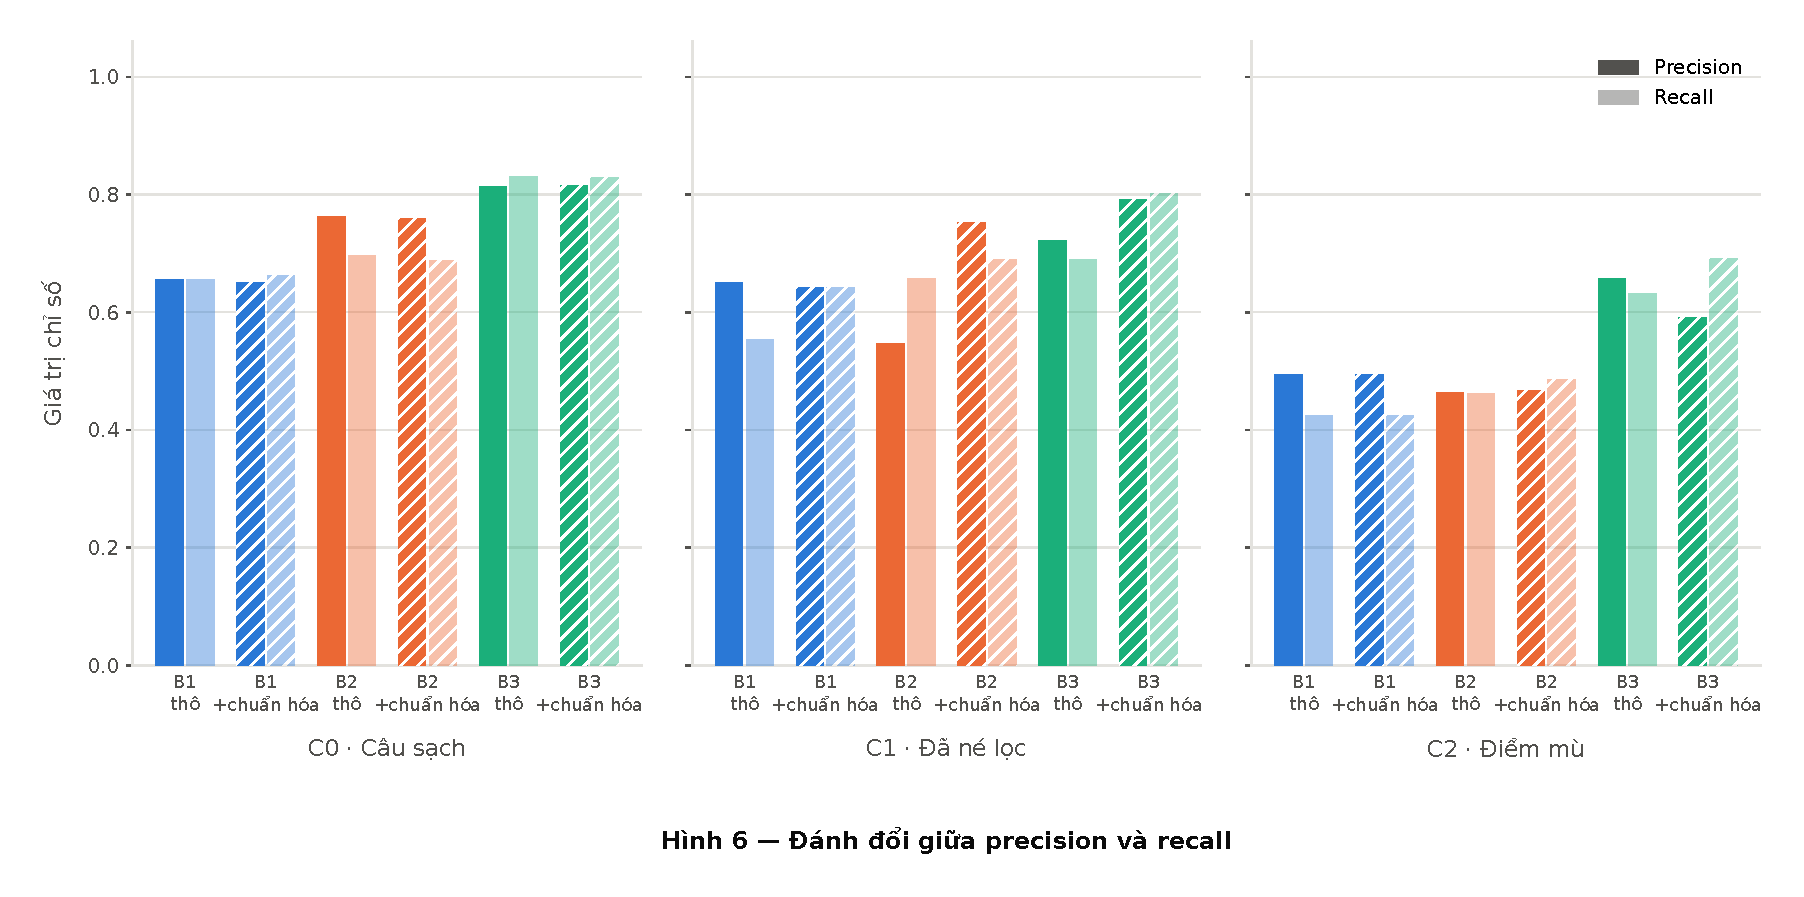
\includegraphics[width=0.88\textwidth]{../results/step3/figures/hinh6_precision_recall.pdf}
\caption{Quan hệ Precision--Recall trong đánh giá}
\label{fig:precision-recall}
\end{figure}

\begin{figure}[H]
\centering
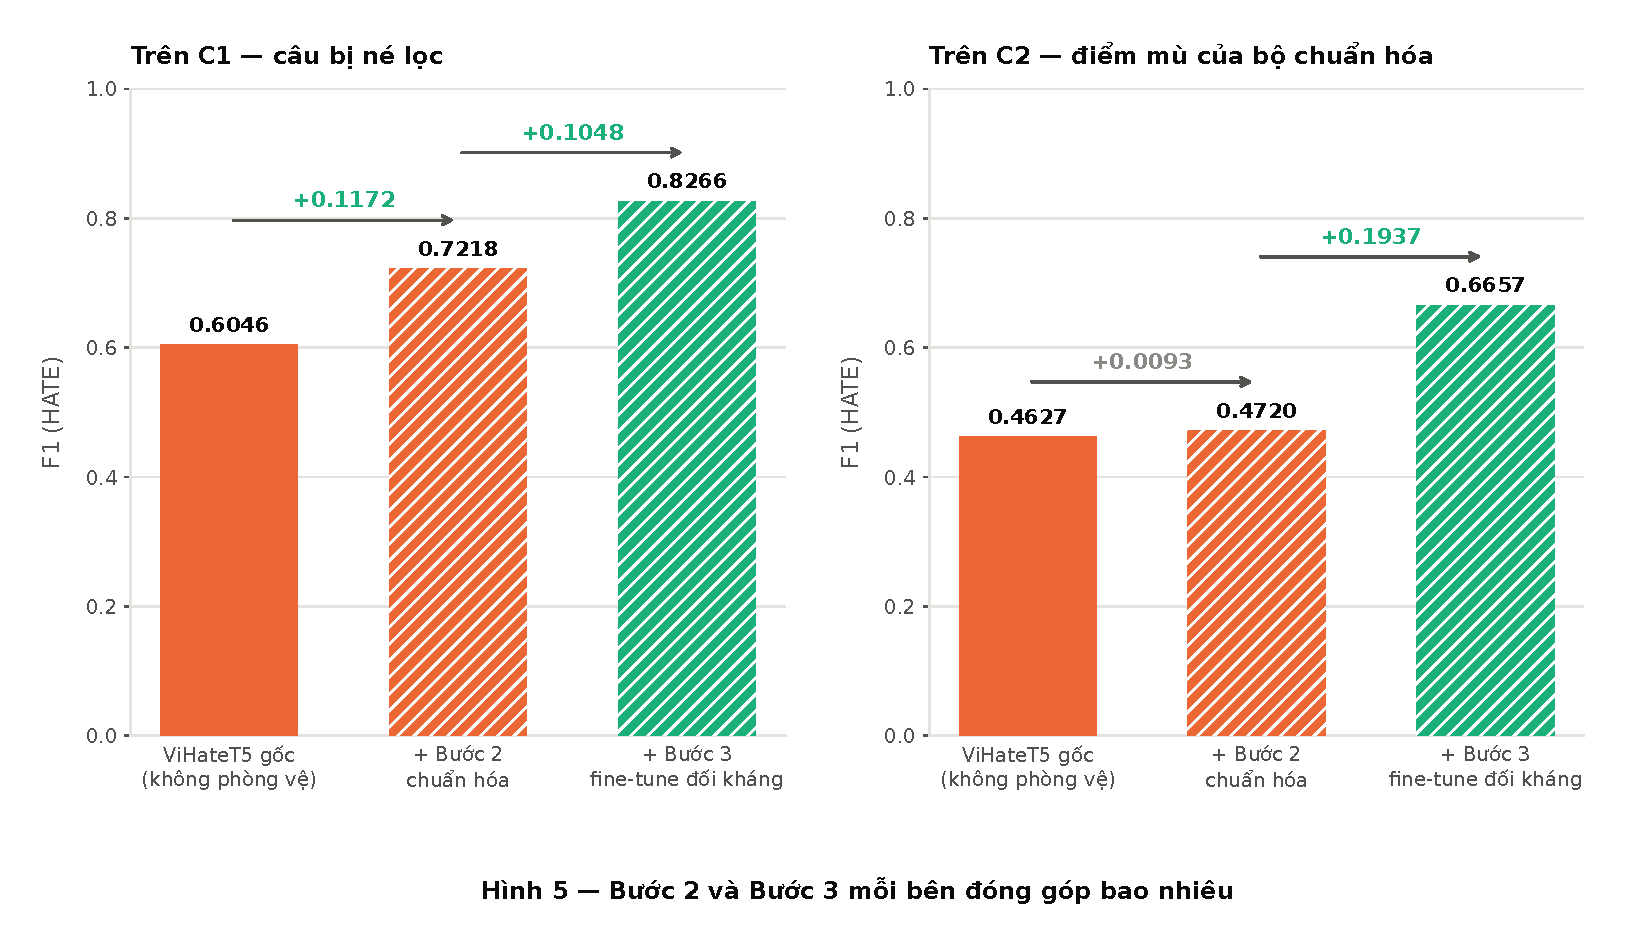
\includegraphics[width=0.88\textwidth]{../results/step3/figures/hinh5_dong_gop_tung_buoc.pdf}
\caption{Mức đóng góp của từng bước trong pipeline}
\label{fig:contribution}
\end{figure}

Hình~\ref{fig:contribution} được dùng để đọc kết quả theo hướng loại bỏ từng thành phần. Chuẩn hóa tạo cải thiện rõ ở C1 vì đưa nhiều biến thể về dạng gần với dữ liệu mà mô hình có thể xử lý. Huấn luyện đối kháng tạo cải thiện lớn hơn ở C2, nơi chuẩn hóa không có tác dụng trực tiếp. Khi ghép cả hai bước, kết quả tăng thêm cho thấy đây là các cơ chế bổ trợ chứ không phải hai phương án thay thế.

\begin{figure}[H]
\centering
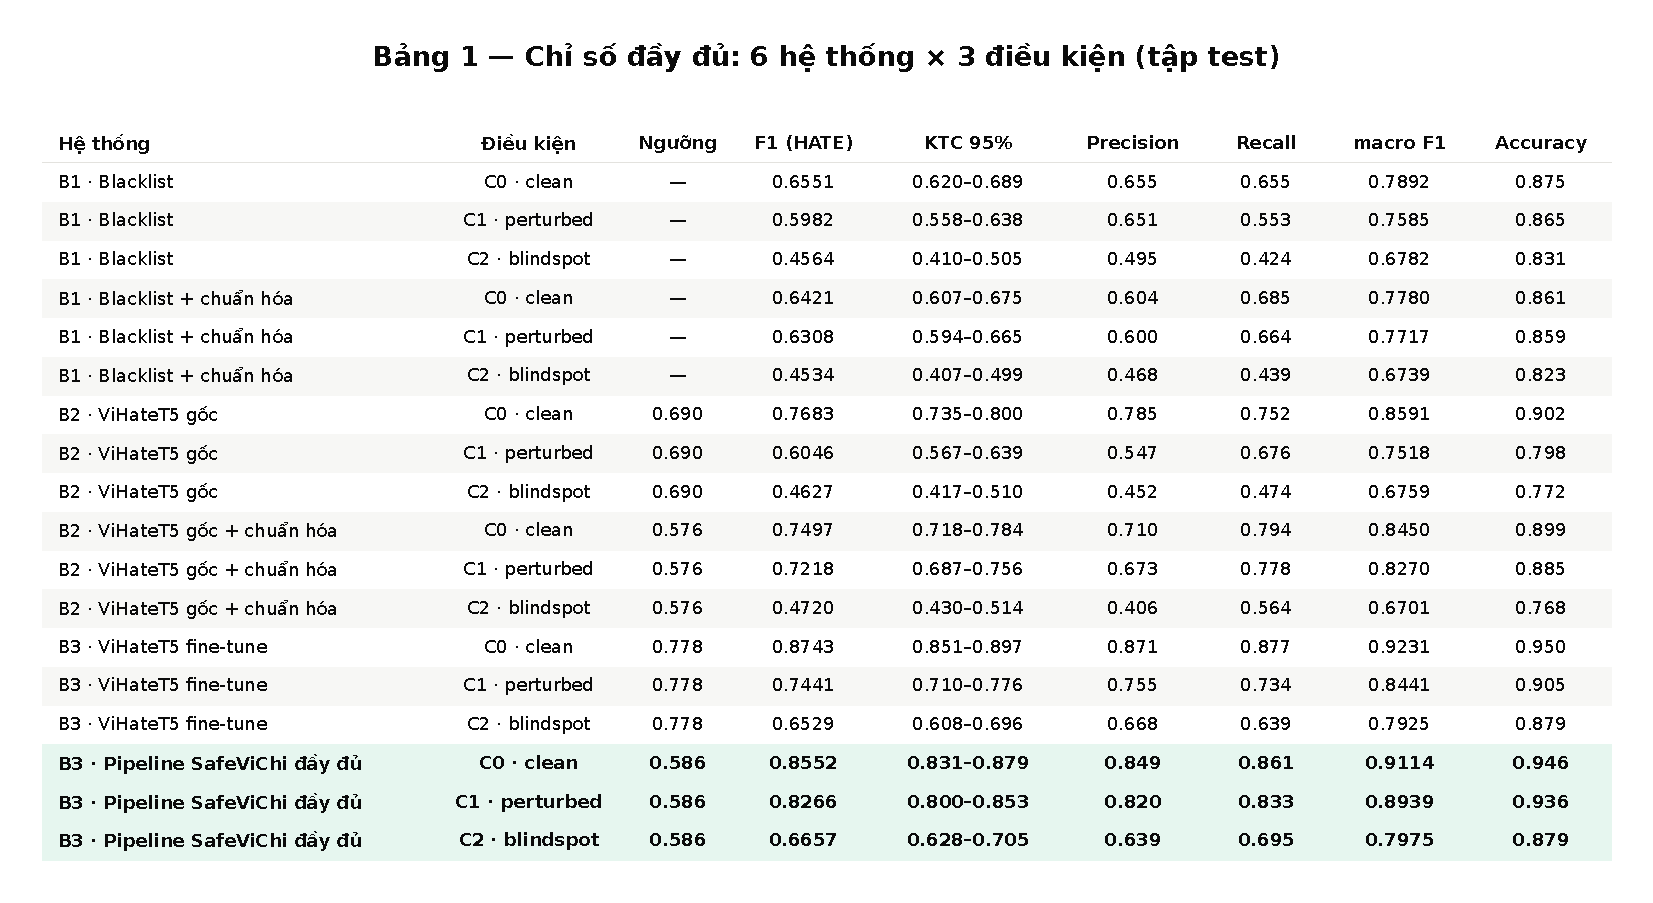
\includegraphics[width=0.88\textwidth]{../results/step3/figures/bang1_chi_so_day_du.pdf}
\caption{Bảng chỉ số đầy đủ của các hệ thống trong thực nghiệm}
\label{fig:full-metrics}
\end{figure}

Bảng chỉ số đầy đủ ở Hình~\ref{fig:full-metrics} cung cấp thông tin bổ sung cho F1, gồm Precision, Recall, accuracy và các chỉ số theo từng điều kiện. Đây là cơ sở để phân biệt hai hệ thống có F1 gần nhau nhưng hành vi khác nhau: một hệ thống có thể ưu tiên Recall để giảm bỏ sót, trong khi hệ thống còn lại ưu tiên Precision để giảm cảnh báo nhầm. Khi đưa vào môi trường thực tế, lựa chọn ngưỡng cần dựa trên chi phí của hai loại sai sót chứ không chỉ dựa trên điểm trung bình.

\begin{figure}[H]
\centering
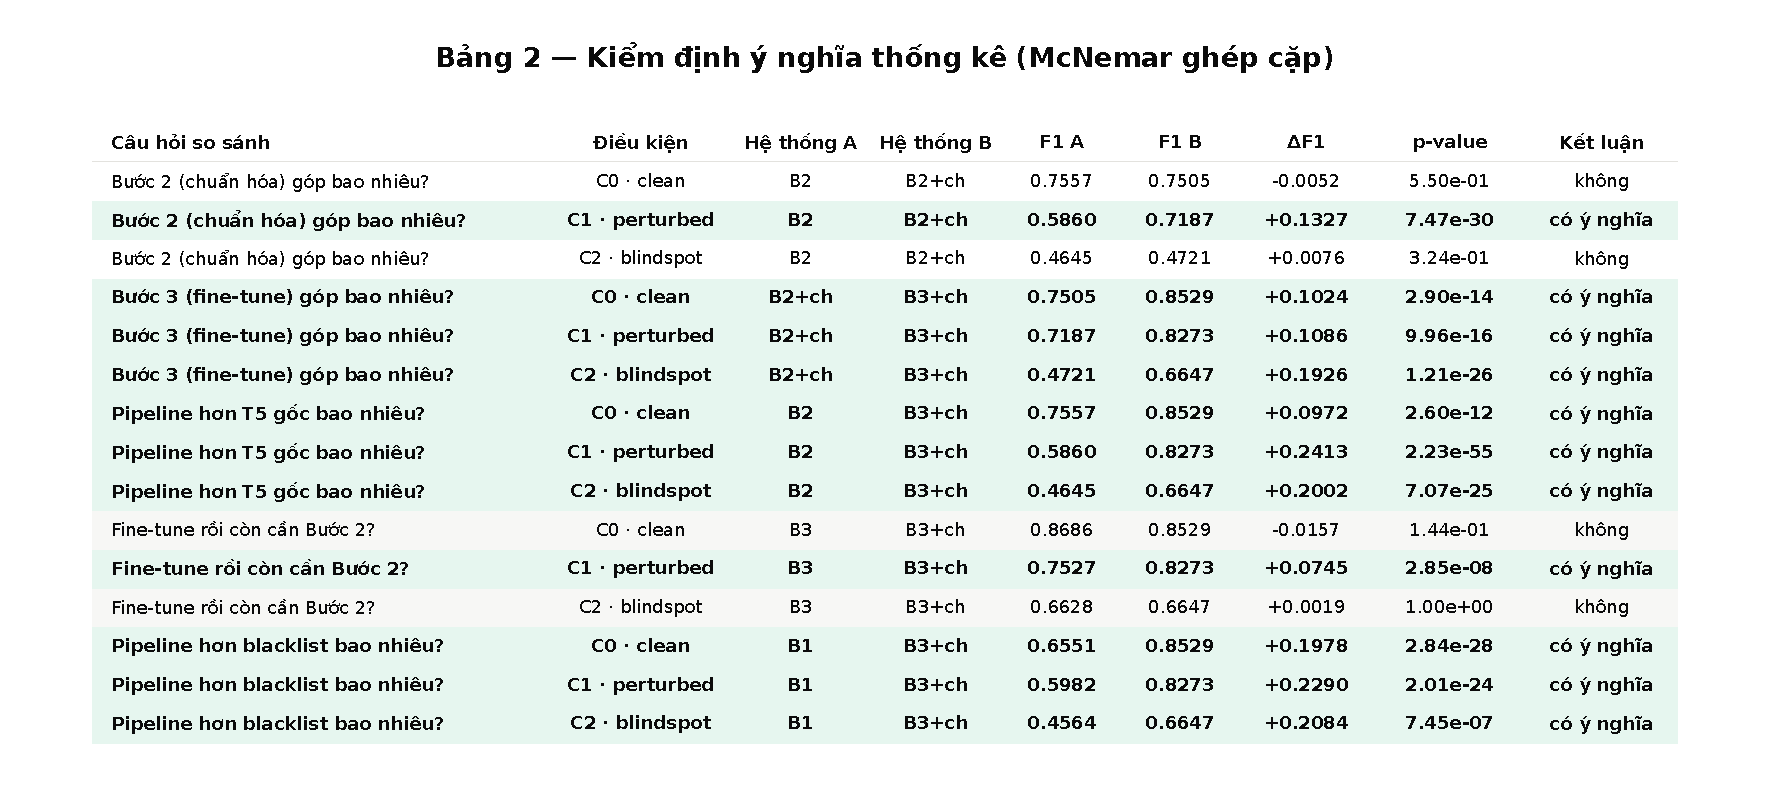
\includegraphics[width=0.88\textwidth]{../results/step3/figures/bang2_mcnemar.pdf}
\caption{Kết quả kiểm định McNemar giữa các cấu hình}
\label{fig:mcnemar}
\end{figure}

Hình~\ref{fig:mcnemar} trình bày kiểm định ghép cặp trên cùng các mẫu. Kiểm định này phù hợp với benchmark vì mỗi hệ thống được chạy trên cùng câu và cùng điều kiện, thay vì so sánh hai mẫu độc lập. Kết quả thống kê không thay thế cho phân tích kỹ thuật, nhưng giúp xác định các chênh lệch quan sát được có đủ bằng chứng để xem là cải thiện có ý nghĩa trong tập thử nghiệm hay không.

\subsection{Đọc kết quả theo điều kiện vận hành}
Ở điều kiện C0, mục tiêu là duy trì khả năng phân loại thông thường và tránh làm giảm hiệu năng do tiền xử lý. Ở C1, mục tiêu là khôi phục tín hiệu sau những thay đổi hình thức có thể mô tả bằng luật hoặc gặp trong dữ liệu sinh. Ở C2, mục tiêu là đo khả năng của mô hình khi không thể dựa vào normalizer. Việc tách ba điều kiện giúp tránh kết luận sai rằng một mô hình tốt trên câu sạch đương nhiên chống được né lọc.

Kết quả cũng cho thấy không nên đánh giá hệ thống chỉ bằng độ chính xác tổng thể. Nếu lớp CLEAN chiếm đa số, một hệ thống dự đoán quá thận trọng có thể đạt accuracy cao nhưng bỏ sót nhiều câu HATE. Vì vậy, hồ sơ sử dụng F1 của lớp HATE làm chỉ số trung tâm, đồng thời báo cáo Precision, Recall, macro F1 và đường cong theo ngưỡng để mô tả đầy đủ hơn.

\subsection{Ưu điểm}
\begin{itemize}
  \item Kết hợp hai cơ chế bổ trợ: chuẩn hóa theo luật xử lý các dạng biến đổi đã biết, còn huấn luyện đối kháng tăng độ bền trước dạng biến đổi tinh vi và điểm mù.
  \item Có đánh giá tách C0, C1 và C2, vì vậy mức suy giảm do né lọc được quan sát trực tiếp thay vì chỉ báo cáo một điểm trung bình.
  \item Xử lý cục bộ giúp giảm rủi ro lộ nội dung văn bản trong quá trình suy luận.
  \item Có module giải thích khoanh vùng, hỗ trợ kiểm tra lý do cảnh báo thay vì chỉ trả về một nhãn.
  \item Pipeline, manifest, seed, mã băm và bộ kiểm thử giúp tái lập các bước dựng dữ liệu và đánh giá.
\end{itemize}

\subsection{Hạn chế}
\begin{itemize}
  \item C2 vẫn thấp hơn C0 và C1; các biến thể được thiết kế để vượt qua chuẩn hóa là giới hạn có chủ đích của phương pháp.
  \item Precision của module giải thích thấp hơn Recall do cửa sổ occlusion có thể bao phủ cả từ lân cận.
  \item ViHateT5 và checkpoint ONNX có thể yêu cầu bộ nhớ, thời gian khởi tạo và năng lực tính toán đáng kể trên thiết bị yếu.
  \item Chất lượng mô hình phụ thuộc vào phạm vi nhãn và hiện tượng biến dạng có trong dữ liệu huấn luyện; các ngữ cảnh mới vẫn cần được đánh giá riêng.
\end{itemize}

\subsection{Khả năng mở rộng}
Có thể mở rộng hệ thống bằng cách bổ sung hiện tượng biến dạng mới, cập nhật từ điển teencode theo phiên bản, thêm dữ liệu có kiểm duyệt và xuất các phiên bản ONNX tối ưu theo nhóm thiết bị. Cách chia module cho phép thay thế bộ phân loại hoặc module giải thích mà không phải viết lại toàn bộ giao diện. Khi mở rộng, cần giữ ma trận C0/C1/C2, kiểm tra rò rỉ dữ liệu và đánh giá lại ngưỡng trên validation mới.

\subsection{Phân tích các dạng sai số}
Sai số của hệ thống có thể chia thành bốn nhóm. Nhóm thứ nhất là câu HATE bị bỏ sót vì biến dạng làm mất tín hiệu mà normalizer chưa có luật xử lý. Nhóm thứ hai là câu CLEAN bị cảnh báo do mô hình dựa quá nhiều vào từ khóa hoặc cụm từ có hình thức giống nội dung HATE. Nhóm thứ ba là lỗi ranh giới trong module giải thích, khi vùng dự đoán bao phủ thêm từ lân cận. Nhóm thứ tư là lỗi vận hành, chẳng hạn mô hình chưa tải xong, văn bản vượt giới hạn đầu vào hoặc tệp ONNX không tương thích.

Với nhóm bỏ sót, hướng xử lý phù hợp là bổ sung biến thể vào tập huấn luyện, không chỉ thêm từ khóa vào blacklist. Với nhóm cảnh báo nhầm, cần xem lại ngữ cảnh, nhãn dữ liệu và ngưỡng; hạ ngưỡng để tăng Recall có thể làm Precision giảm. Với lỗi giải thích, có thể thử cửa sổ nhỏ hơn hoặc hậu xử lý vùng liền kề, nhưng mọi thay đổi phải được đánh giá lại trên validation và test tương ứng.

Một điểm cần giữ nguyên là phân biệt lỗi mô hình với lỗi dữ liệu. Nếu câu nguồn bị gán nhãn không nhất quán, việc thay đổi kiến trúc không chắc giải quyết được vấn đề. Vì vậy, các mẫu có điểm thấp hoặc bất đồng giữa hệ thống nên được đưa vào danh sách xem xét, nhưng không tự động đổi nhãn test sau khi đã công bố kết quả. Việc sửa dữ liệu phải tạo phiên bản mới và chạy lại toàn bộ giao thức.

\subsection{Khả năng mở rộng theo quy mô dữ liệu}
Khi số lượng dữ liệu tăng, bước sinh biến thể và bước tokenization có thể được chạy theo lô. Các tệp JSON Lines cho phép xử lý tuần tự, còn manifest cho phép theo dõi tiến độ và nối kết quả. Để tránh tăng chi phí không cần thiết, có thể ưu tiên sinh thêm những dạng biến thể mà F1 C1 hoặc C2 đang thấp, thay vì chỉ tăng ngẫu nhiên số lượng câu.

Khi mở rộng sang miền dữ liệu mới, cần thu thập một tập validation đại diện cho miền đó trước khi điều chỉnh ngưỡng. Một mô hình có thể đạt kết quả tốt trên dữ liệu mạng xã hội nhưng suy giảm trên bình luận trò chơi, diễn đàn hoặc tin nhắn ngắn. Việc báo cáo theo miền và theo dạng biến thể giúp xác định phạm vi áp dụng cụ thể hơn một con số chung.

\section{So sánh với phương án hoặc mô hình cơ sở, phân tích đóng góp của các thành phần trong hệ thống}
\subsection{So sánh với phương án cơ sở}
Blacklist từ khóa có chi phí thấp nhưng phụ thuộc vào việc từ vi phạm xuất hiện nguyên dạng, nên dễ bỏ sót khi văn bản bị biến dạng. ViHateT5 gốc hiểu ngữ cảnh tốt hơn nhưng F1 C1 giảm từ 0,7683 ở C0 xuống 0,6046. Thêm chuẩn hóa giúp F1 C1 tăng lên 0,7218, nhưng chỉ cải thiện hạn chế ở C2. Tinh chỉnh đối kháng giúp mô hình học trực tiếp các phân bố biến dạng; kết hợp cả hai thành phần tạo ra SafeViChi đầy đủ với F1 C1 0,8266.

\begin{table}[H]
\centering
\caption{Đóng góp của các thành phần theo F1 C1}
\label{tab:ablation}
\begin{tabular}{lcc}
\toprule
\textbf{Cấu hình} & \textbf{F1 C1} & \textbf{Thay đổi so với ViHateT5 gốc}\\
\midrule
ViHateT5 gốc & 0,6046 & --\\
ViHateT5 gốc + chuẩn hóa & 0,7218 & +0,1172\\
Tinh chỉnh đối kháng, không chuẩn hóa & 0,7441 & +0,1395\\
SafeViChi đầy đủ & 0,8266 & +0,2220\\
\bottomrule
\end{tabular}
\end{table}

\subsection{Phân tích đóng góp}
Lớp chuẩn hóa có đóng góp trực tiếp và dễ kiểm tra đối với các dạng biến thể nằm trong phạm vi luật. Huấn luyện đối kháng làm giảm sự phụ thuộc của mô hình vào hình thức bề mặt và tạo cải thiện rõ ở C2. Hai thành phần không thay thế nhau: khi kết hợp, chuẩn hóa giảm độ phức tạp của đầu vào ở các trường hợp đã biết, còn mô hình xử lý phần dư và các trường hợp chưa được luật bao phủ. Module occlusion không làm thay đổi nhãn phân loại; nó bổ sung khả năng kiểm tra và giải thích kết quả.

Ngoài bảng loại bỏ thành phần, có thể đọc đóng góp qua thời điểm hoạt động. Blacklist và normalizer có thể xử lý một số trường hợp với chi phí tính toán thấp, nhưng không mô hình hóa được ngữ cảnh dài. ViHateT5 cung cấp năng lực hiểu ngữ cảnh nhưng chịu ảnh hưởng của biến dạng. FGM chỉ hoạt động trong lúc huấn luyện, song tác động của nó thể hiện ở độ bền của checkpoint sau khi triển khai. Occlusion làm tăng số lần suy luận khi cần giải thích, do đó nên bật theo nhu cầu hoặc chỉ chạy với các câu đã được gắn cờ.

Hệ thống vì vậy có thể được vận hành theo hai mức. Mức nhanh trả về nhãn và điểm rủi ro bằng chuẩn hóa cộng mô hình. Mức kiểm tra mở rộng chạy occlusion để trả về vùng cảnh báo. Cách phân tầng này cân bằng giữa thời gian phản hồi và nhu cầu giải thích trong các tình huống kiểm duyệt, nghiên cứu hoặc kiểm tra nội dung.

So sánh này cũng chỉ ra sự khác nhau về chi phí vận hành. Blacklist có thể chạy rất nhanh nhưng chi phí bảo trì từ khóa tăng theo phạm vi nội dung và không giải quyết được biến dạng mới. Mô hình nền yêu cầu nhiều tài nguyên hơn nhưng có khả năng sử dụng ngữ cảnh. Lớp chuẩn hóa tăng một lượng xử lý nhỏ trước suy luận, còn FGM làm tăng chi phí ở giai đoạn huấn luyện chứ không tạo thêm một bước nặng khi chạy dự đoán. Occlusion là thành phần có chi phí suy luận cao nhất vì cần chạy lại mô hình cho nhiều cửa sổ từ.

Đóng góp của hệ thống vì vậy không chỉ được đo bằng F1. SafeViChi kết hợp khả năng phát hiện, chống né lọc, giải thích và xử lý cục bộ trong cùng pipeline. Khi triển khai ở nơi yêu cầu thời gian phản hồi thấp, có thể chỉ chạy hai tầng đầu ra nhãn và điểm rủi ro. Khi cần kiểm duyệt hoặc phân tích sau sự kiện, có thể chạy thêm occlusion cho các mẫu HATE hoặc mẫu có điểm gần ngưỡng.

\section{Kiến trúc hệ thống và phương án triển khai}
\subsection{Kiến trúc xử lý}
Hệ thống gồm bốn tầng chính như Hình~\ref{fig:architecture}: chuẩn bị dữ liệu, chuẩn hóa, phân loại và giải thích. Ở chế độ sản phẩm, ba tầng cuối chạy phía trình duyệt.

\begin{figure}[H]
\centering
\fbox{\begin{minipage}{0.92\textwidth}
\centering
\vspace{3mm}
\textbf{Văn bản đầu vào}\par\vspace{2mm}
$\downarrow$\par\vspace{2mm}
\fcolorbox{navy}{lightblue}{\parbox{0.72\textwidth}{\centering Chuẩn hóa năm tầng\\Unicode NFC -- ký tự đồng dạng -- phân cách -- lặp ký tự -- teencode}}\par\vspace{3mm}
$\downarrow$\par\vspace{2mm}
\fcolorbox{navy}{lightblue}{\parbox{0.72\textwidth}{\centering ViHateT5 tinh chỉnh đối kháng\\ONNX Runtime Web}}\par\vspace{3mm}
$\downarrow$\par\vspace{2mm}
\fcolorbox{navy}{lightblue}{\parbox{0.72\textwidth}{\centering Nhãn CLEAN/HATE và điểm rủi ro}}\par\vspace{3mm}
$\downarrow$\par\vspace{2mm}
\fcolorbox{navy}{lightblue}{\parbox{0.72\textwidth}{\centering Occlusion khoanh vùng cụm từ cảnh báo}}\\
\vspace{3mm}
\end{minipage}}
\caption{Kiến trúc xử lý của SafeViChi}
\label{fig:architecture}
\end{figure}

\subsection{Luồng xử lý}
Khi người dùng nhập văn bản, bản sao xử lý được chuyển qua normalizer. Chuỗi sau chuẩn hóa được tokenizer và đưa vào mô hình ONNX. Kết quả gồm nhãn và điểm rủi ro. Nếu cần giải thích, hệ thống che từng cửa sổ hai từ, chạy lại suy luận và tính mức giảm logit margin để đánh dấu các cụm có ảnh hưởng lớn. Không có bước nào yêu cầu gửi nội dung đến dịch vụ suy luận bên ngoài.

\subsection{Phương án triển khai}
Trong môi trường thử nghiệm, chạy máy chủ tệp nội bộ bằng lệnh \texttt{python -m http.server 8000} tại thư mục \sourcepath{demo/}. Người dùng mở giao diện bằng trình duyệt và có thể kiểm tra tab Network để xác nhận không phát sinh request chứa văn bản đến máy chủ ứng dụng. Trong môi trường thực tế, có thể đóng gói giao diện và mô hình ONNX trong ứng dụng web nội bộ, ứng dụng máy tính hoặc ứng dụng di động có lớp thực thi ONNX tương ứng. Việc cập nhật mô hình nên dùng phiên bản có mã kiểm tra và kiểm thử hồi quy trên ma trận C0/C1/C2.

\subsection{Yêu cầu tài nguyên và kiểm soát phiên bản}
Lần chạy huấn luyện cần GPU; tài liệu pipeline ghi nhận cấu hình tham khảo hai GPU Nvidia T4 và thời gian khoảng năm đến sáu giờ. Đánh giá ma trận đầy đủ cũng cần GPU, trong khi module occlusion có thể chạy trên CPU nhưng mất nhiều thời gian hơn do phải suy luận nhiều lần. Demo trình duyệt cần tải tokenizer, tệp cấu hình và mô hình ONNX trước lần suy luận đầu tiên, vì vậy giao diện phải có trạng thái đang tải và trạng thái lỗi rõ ràng.

Mỗi bản phát hành nên gắn với phiên bản của từ điển, normalizer, tokenizer, checkpoint và cấu hình ngưỡng. Khi một thành phần thay đổi, cần chạy lại tối thiểu bộ hồi quy gồm câu sạch, các dạng né lọc phổ biến, câu điểm mù và các ví dụ có giải thích. Kết quả phải được lưu cùng seed và mã băm để phân biệt cải thiện thật với thay đổi do dữ liệu hoặc môi trường.

\subsection{Luồng triển khai theo môi trường}
Trong giai đoạn phát triển, mô hình PyTorch được dùng để huấn luyện và đánh giá chi tiết. Trong giai đoạn trình diễn, bản ONNX và giao diện tĩnh được phục vụ bởi một máy chủ tệp nội bộ. Trong giai đoạn tích hợp, có thể đưa cùng giao diện vào một ứng dụng không kết nối mạng hoặc một ứng dụng nội bộ có chính sách bảo vệ dữ liệu. Nếu cần cập nhật mô hình từ xa, chỉ tải gói đã ký hoặc đã kiểm tra mã băm; việc cập nhật không được làm thay đổi ngưỡng mà không tạo phiên bản đánh giá mới.

\section{Phân tích rủi ro, yêu cầu bảo mật, đạo đức trí tuệ nhân tạo và an toàn dữ liệu}
\subsection{Rủi ro có thể phát sinh}
\begin{itemize}
  \item \textbf{Bỏ sót nội dung độc hại}: biến thể mới hoặc ngữ cảnh chưa có trong dữ liệu có thể làm mô hình dự đoán CLEAN. C2 được xây dựng để đo một phần rủi ro này.
  \item \textbf{Cảnh báo nhầm}: câu trích dẫn, câu đùa hoặc cách dùng từ trong ngữ cảnh đặc biệt có thể bị đánh dấu HATE. Cảnh báo phải được xem là tín hiệu hỗ trợ, không phải kết luận cuối cùng.
  \item \textbf{Thiên lệch dữ liệu}: nhãn do con người gán và nguồn dữ liệu có thể phản ánh thiên kiến về vùng miền, cách nói hoặc nhóm người. Cần ghi nhận nguồn, rà soát mẫu bất thường và không dùng một điểm số duy nhất để đánh giá công bằng.
  \item \textbf{Rủi ro riêng tư}: log, ảnh chụp màn hình hoặc dữ liệu trung gian có thể vô tình chứa văn bản người dùng. Mọi minh chứng phải được làm sạch trước khi chia sẻ.
  \item \textbf{Rủi ro lạm dụng}: mô hình có thể bị dùng để giám sát quá mức hoặc tự động chặn người dùng. Quy trình triển khai cần giữ quyền xem xét và quyết định cuối cùng của con người.
  \item \textbf{Rủi ro vận hành}: mô hình hoặc tokenizer không tải đủ, thiết bị thiếu bộ nhớ, phiên bản ONNX không tương thích hoặc văn bản quá dài có thể làm hệ thống không trả kết quả.
\end{itemize}

\subsection{Yêu cầu bảo mật và an toàn dữ liệu}
\begin{itemize}
  \item Văn bản đầu vào được chuẩn hóa và suy luận trong trình duyệt; không thiết kế đường truyền văn bản đến máy chủ bên ngoài.
  \item Chỉ lưu những thông tin cần cho phiên sử dụng. Không lưu lâu dài văn bản, không ghi văn bản nguyên bản vào nhật ký lỗi và cần xóa bộ nhớ tạm sau khi kết thúc phiên.
  \item Mô hình, từ điển và tệp cấu hình phải được kiểm tra mã băm trước khi sử dụng để tránh chạy tệp bị thay thế.
  \item Dữ liệu huấn luyện, kết quả thử nghiệm và ảnh minh chứng phải được phân quyền. Các tệp chia sẻ công khai không được chứa mật khẩu, khóa truy cập, token hoặc dữ liệu cá nhân.
  \item Khi cập nhật mô hình, phải giữ phiên bản, mã băm, ngưỡng và kết quả kiểm thử hồi quy để có thể truy nguyên thay đổi.
\end{itemize}

\subsection{Đạo đức trí tuệ nhân tạo và kiểm soát đầu ra}
SafeViChi chỉ đưa ra nhãn và cảnh báo xác suất, không tự động xử phạt, xóa nội dung hoặc kết luận về một cá nhân. Người vận hành cần được biết giới hạn của mô hình, điều kiện dữ liệu và khả năng sai. Vùng tô sáng từ module giải thích chỉ là bằng chứng hỗ trợ, không được trình bày như nguyên nhân chắc chắn theo nghĩa pháp lý.

Khi dùng trong môi trường giáo dục, cần thông báo rõ mục đích sử dụng, giới hạn thu thập dữ liệu và quyền được giải thích. Cần ưu tiên cảnh báo có thể kiểm tra, cho phép người dùng phản hồi và có cơ chế xem xét lại trường hợp bị cảnh báo nhầm. Việc đánh giá định kỳ nên theo dõi riêng Recall, Precision theo nhóm dữ liệu và các trường hợp sai nghiêm trọng, thay vì chỉ theo dõi F1 trung bình.

\section{Hướng phát triển, hoàn thiện và khả năng ứng dụng trong thực tiễn}
\subsection{Hiện trạng và bước hoàn thiện gần nhất}
Phiên bản hiện tại đã có pipeline dựng dữ liệu, bộ chuẩn hóa, mô hình ViHateT5 tinh chỉnh đối kháng, module giải thích, checkpoint ONNX và giao diện chạy trong trình duyệt. Bước hoàn thiện gần nhất là đóng gói bản trình diễn ổn định, bổ sung kiểm thử trên các thiết bị có cấu hình khác nhau và ghi nhận thời gian tải mô hình, thời gian suy luận cũng như mức sử dụng bộ nhớ.

\subsection{Hướng phát triển kỹ thuật}
\begin{itemize}
  \item Mở rộng tập dữ liệu bằng các biến thể mới, dữ liệu nhiều miền và các mẫu do người kiểm duyệt xác nhận; giữ nguyên quy trình khử trùng lặp và chống rò rỉ.
  \item Xây dựng vòng cập nhật benchmark để theo dõi các kỹ thuật né lọc mới thay vì chỉ dựa vào từ điển tĩnh.
  \item Tối ưu bản ONNX theo thiết bị, giảm thời gian khởi động và cung cấp cơ chế tải mô hình có kiểm tra mã băm.
  \item Cải thiện module giải thích bằng cách khảo sát cửa sổ từ khác nhau và phương pháp hậu xử lý biên, nhưng chỉ phát hành sau khi đánh giá lại trên tập có nhãn.
  \item Bổ sung kiểm thử độ bền, kiểm thử riêng tư và kiểm thử hồi quy tự động cho giao diện, tokenizer, normalizer và mô hình.
  \item Xây dựng cơ chế phản hồi của người dùng có kiểm duyệt, trong đó mẫu phản hồi được ẩn danh và chỉ đưa vào huấn luyện sau khi được xem xét.
\end{itemize}

\subsection{Khả năng ứng dụng thực tiễn}
Trong giáo dục, hệ thống có thể dùng làm công cụ hỗ trợ nhận diện sớm nội dung có nguy cơ trong môi trường học tập trực tuyến. Trong gia đình, hệ thống có thể cung cấp cảnh báo cục bộ mà không cần gửi toàn bộ tin nhắn lên máy chủ. Trong các sản phẩm số, mô hình có thể được tích hợp ở tầng thiết bị hoặc trình duyệt để giảm độ trễ và giảm lượng dữ liệu phải truyền.

Việc áp dụng thực tế cần triển khai theo từng giai đoạn: thử nghiệm nội bộ, đánh giá với người vận hành, kiểm tra sai số và riêng tư, sau đó mới mở rộng phạm vi. Mỗi môi trường phải có chính sách rõ về người được xem cảnh báo, thời gian lưu dữ liệu, cách xử lý khiếu nại và trách nhiệm quyết định. SafeViChi phù hợp nhất với vai trò lớp cảnh báo và hỗ trợ kiểm duyệt, không nên được sử dụng như cơ chế duy nhất để tự động quyết định quyền truy cập hoặc xử lý kỷ luật.

\section{Lịch sử câu lệnh và hình ảnh minh chứng quá trình phát triển sản phẩm từ bản nháp đến khi hoàn thiện}
\subsection{Đường liên kết minh chứng}
\begin{center}
\fbox{\parbox{0.9\textwidth}{\centering
\url{docs/demo-pipeline-terminal-log.txt}}}
\end{center}

\begin{flushright}
  \begin{minipage}{0.68\textwidth}
    \centering
    \vspace{8mm}
    \textbf{Hà Nội, ngày 19 tháng 9 năm 2026}\\
    \textbf{Đại diện đội thi}\\[1mm]
    (Ký, ghi rõ họ tên)\\[1mm]
    \textit{(Đã ẩn chữ ký và họ tên)}
  \end{minipage}
\end{flushright}

\end{document}
